\section{Experimentos y Resultados}
\subsection{Entorno de pruebas e imágenes} %(prototipos) para realizar las pruebas
    \begin{frame}{Definición de imágenes}
      \begin{itemize}
	\item<1-> \textbf{Imagen patrón}: detectar y seguir en cada fotograma del flujo de video. En su lugar se superpone el objeto de realidad aumentada.
	Restricciones prácticas:
	  \begin{enumerate}
	  \item \small tamaño de $640 \times 480$ píxeles,
	  \item \small condiciones de iluminación adecuadas,
	  \item \small imagen debe ser rica en detalles,
	  \item \small plano de la imagen perpendicular al lente de la cámara al momento de la captura.
	  \end{enumerate}

	\item<2-> \textbf{Imagen objetivo}: es un fotograma del flujo de video, adquirido con la cámara web en tiempo real.
	
	\item<3-> \textbf{Objeto de realidad aumentada}: imagen, video, texto, etc. \note[item]{no visual: sonido, plano de un objeto 3d}
      \end{itemize}
    \end{frame}
    
    \begin{frame}{Herramientas}
      \begin{block}{Software}
	\begin{itemize}
	 \item OpenCV 2.3.1.
	 \item C$\slash$C++.
	\end{itemize}
      \end{block}
      \begin{block}{Hardware}
	\begin{itemize}
	  \item Webcam: Resolución de $640 \times 480$ píxeles.
	  \item Procesador Intel® Core 2 Duo 2.2 Ghz., 4Gb. RAM.
	\end{itemize}
      \end{block}
    \end{frame}

    \begin{frame}{Imagen patrón y condiciones de iluminación}
      \begin{itemize}
	\item Imagen patrón: tapa de una revista de $22 \times 17$ cm.
	\item Tres condiciones de iluminación diferentes:
	\begin{enumerate}
	  \item<1-> \textbf{Iluminación normal $(B_{N})$}: 
		\begin{itemize}
		  \item lámpara de bajo consumo de 18 W (90 W. de una lámpara incandescente).
		\end{itemize}
    
	  \item<2-> \textbf{Iluminación alta $(B_{H})$}: 
		  \begin{itemize}
		  \item $(B_{N})$ + iluminación direccional con lámpara incandescente de 60 W.
		  \end{itemize}
	      
	  \item<3-> \textbf{Iluminación baja $(B_{L})$}:
		  \begin{itemize}
		    \item Dificultad para la lectura de un documento.
		    \item Lámparas apagadas.
		  \end{itemize}  
	\end{enumerate}
      \end{itemize}
    \end{frame}
  
  \begin{frame}{Entorno ambiental}
      \begin{figure}[tbhp]
	\centering
	      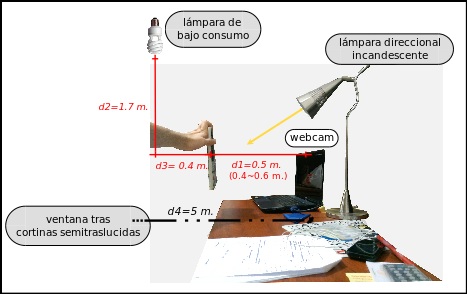
\includegraphics[scale=0.45]{../../figs/entorno/entorno_pruebas_slide}
	  \caption*{Esquema del ambiente en el que se realizaron las pruebas.}
	\label{fig:entorno_pruebas}
      \end{figure}
  \end{frame}
    
\subsection{Experimentos}%Pruebas realizadas
\begin{frame}{Experimentos}
  \begin{block}{Experimento 1: costo computacional y detección de puntos}
  Evaluación del costo computacional y detección de puntos claves bajo las condiciones de iluminación $B_{N}$, $B_{H}$ y $B_{L}$.
  \end{block}
\end{frame}
%%%%%%%%%%%%%%%%%%%%%%%%%%%%%%%%%%%%%%%%%%%%%%%%%%%%%%%%%%%%%%%%%%%%%%%%%%%%%%%%%%%%%%%%%%%%%%%%%%%
\subsubsection*{Experimento 1}
  \label{subsec:paraqumetros_utilizados}
  
  \begin{frame}{Experimento 1}
   \begin{itemize}
  \item Se capturó la imagen patrón en las tres condiciones de iluminación.
      \begin{figure}[H]
      \centering
      \subfloat[\scriptsize{Imagen patrón con condición $B_{N}$.}]{
\includegraphics[width=0.32\textwidth]{../../exp1/train_normal_BN/train_normal} \label{fig:train_normal}}
      \subfloat[\scriptsize{Imagen patrón con condición $B_{H}$.}]{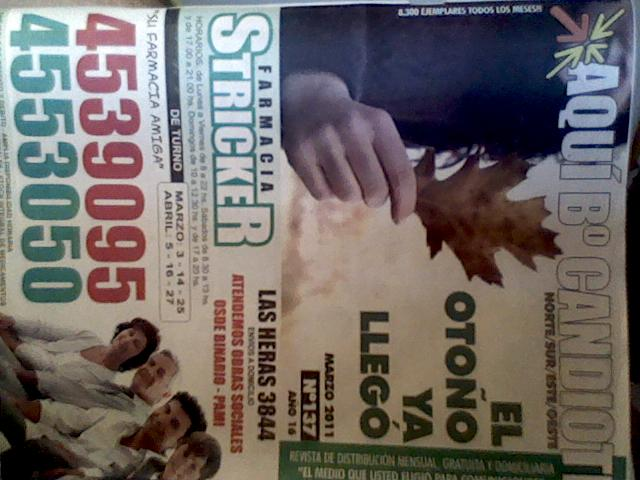
\includegraphics[width=0.32\textwidth]{../../exp1/train_brillante_BH/train_brillante} \label{fig:train_brillante}}
      \subfloat[\scriptsize{Imagen patrón con condición $B_{L}$.}]{
\includegraphics[width=0.32\textwidth]{../../exp1/train_oscura_BL/train_oscura} \label{fig:train_oscura}}
      \caption*{Imágenes obtenidas para condiciones de iluminación diferentes.}
      \label{fig:prueba_iluminacion_realce_detalles_2_imagenes}
    \end{figure}
  \item Se aplicó a cada una de las imágenes operaciones para realce de detalles y mejora en la iluminación.
 \end{itemize}
  \end{frame}
  
  

% \begin{frame}{Condición $B_{N}$}
% \note[item]{\textit{filtrado pasa altos}, \textit{filtro de alta potencia} $\rightarrow$ realza los detalles}
% \note[item]{\textit{ecualización} $\rightarrow$ mejora el contraste}
%   \begin{figure}
%     \centering
%     \subfloat[\tiny{Imagen patrón con Ilum. $B_{N}$}]{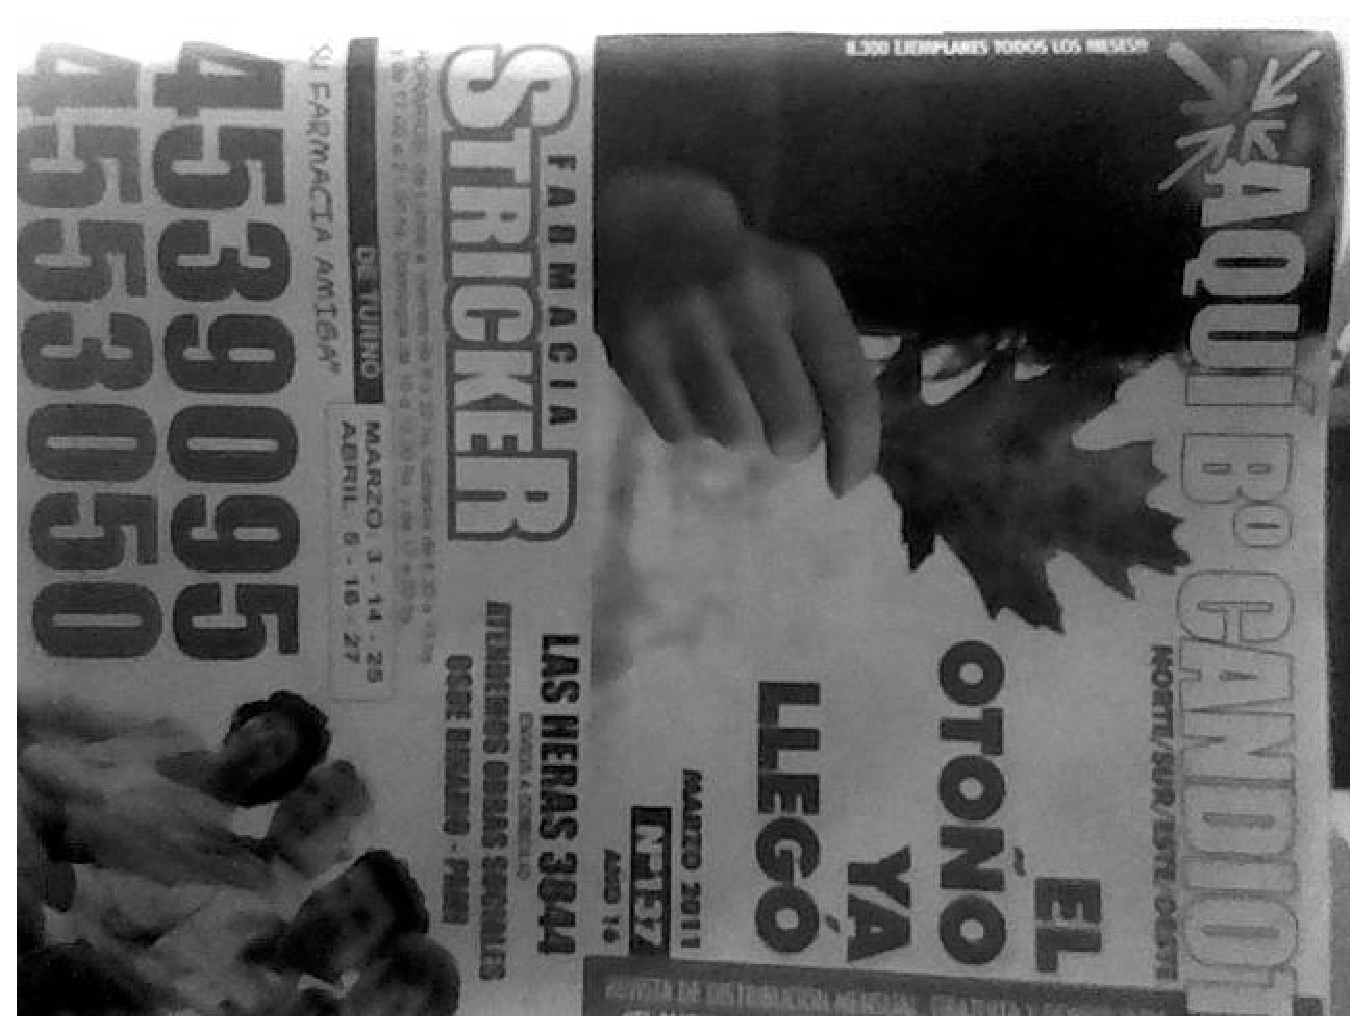
\includegraphics[width=0.32\textwidth]{../../exp1/train_normal_BN/train_normal_grises} \label{fig:iluminacion_BN_original}}
%     \subfloat[\tiny{Transformación logarítmica}]{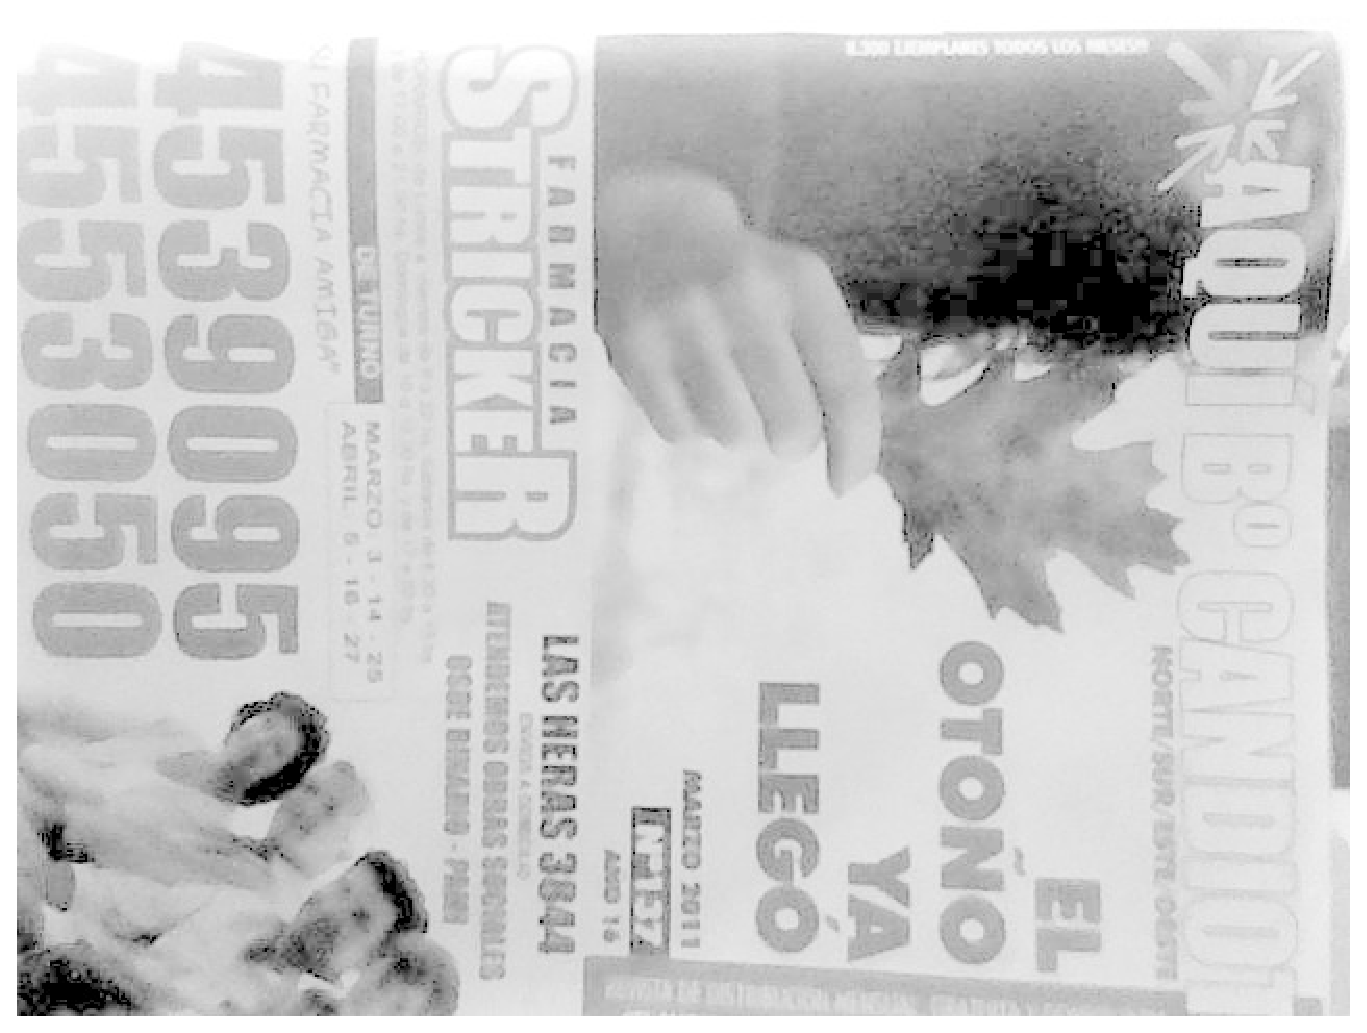
\includegraphics[width=0.32\textwidth]{../../exp1/train_normal_BN/train_normal_515} \label{fig:iluminacion_BN_logaritmica}}
%     \subfloat[\tiny{Ecualización}]{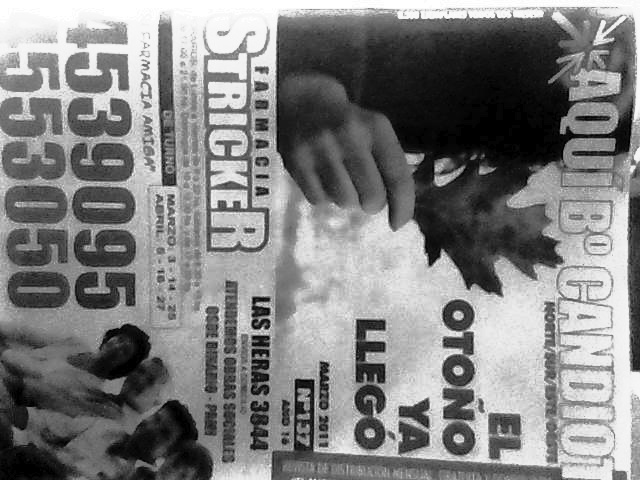
\includegraphics[width=0.32\textwidth]{../../exp1/train_normal_BN/keypoints2} \label{fig:iluminacion_BN_ecualizacion}}\\
%     \subfloat[\tiny{Filtrado pasa altos}]{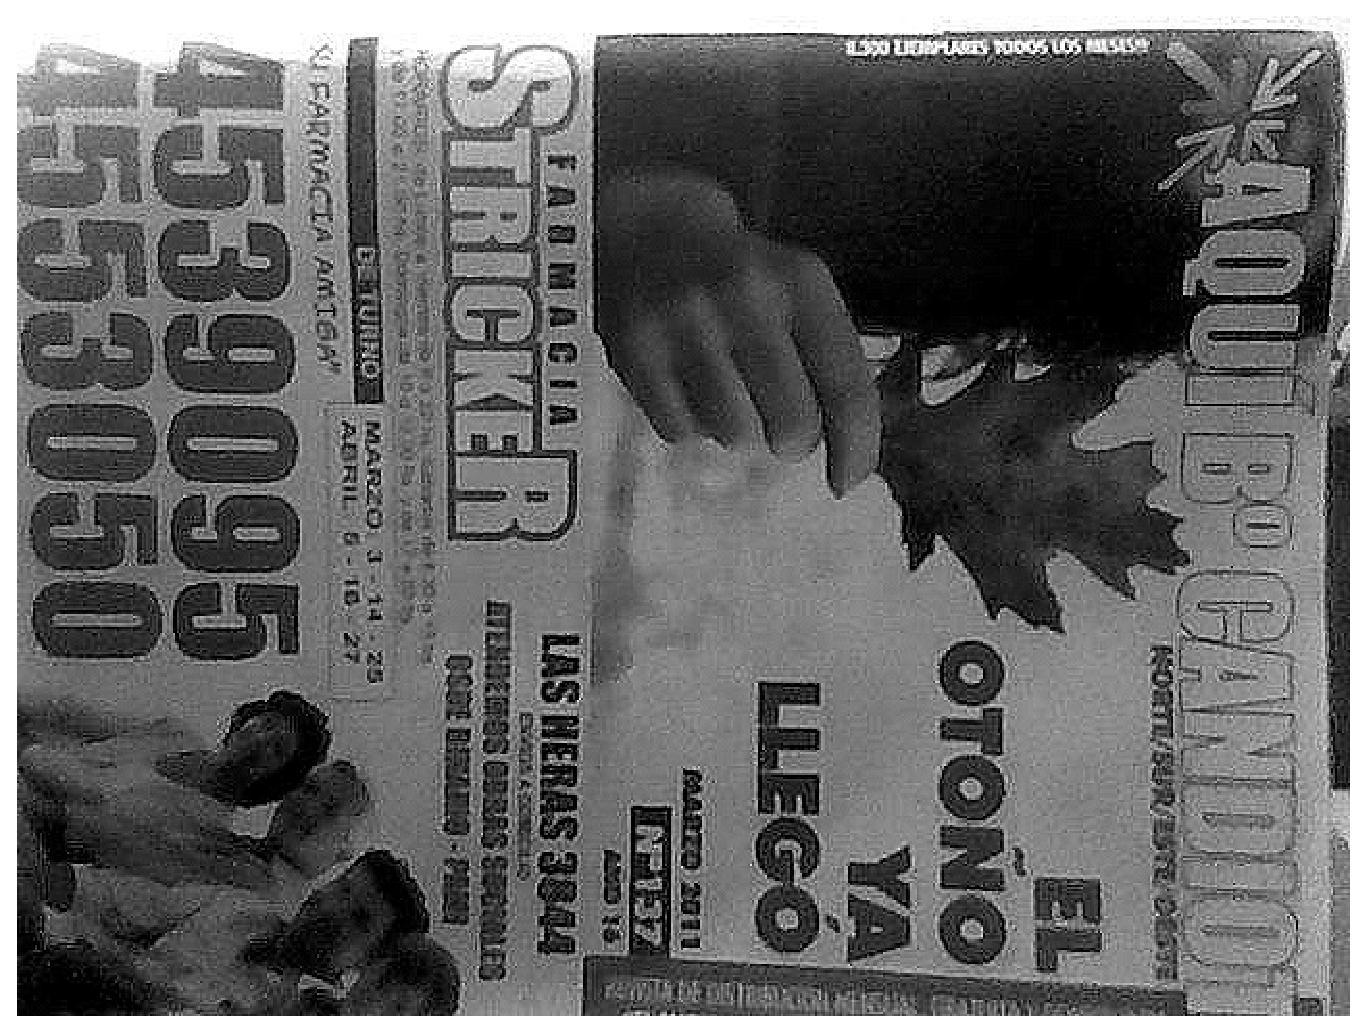
\includegraphics[width=0.32\textwidth]{../../exp1/train_normal_BN/keypoints3} \label{fig:iluminacion_BN_pasaaltos}}
%     \subfloat[\tiny{Filtrado de alta potencia}]{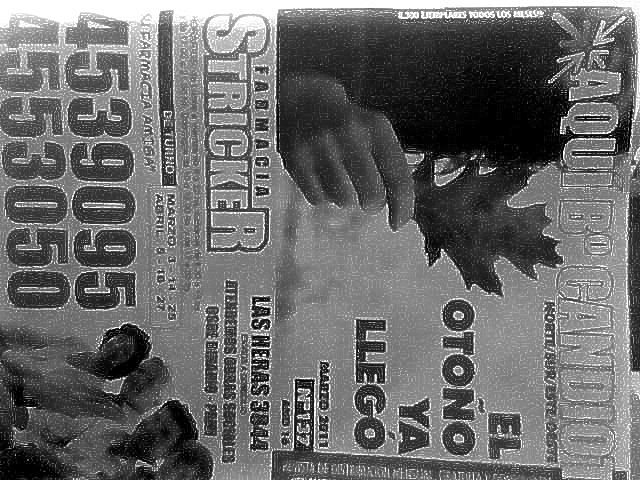
\includegraphics[width=0.32\textwidth]{../../exp1/train_normal_BN/keypoints4} \label{fig:iluminacion_BN_altapotencia}}
%     \subfloat[\tiny{Ecualización + filtrado de alta potencia}]{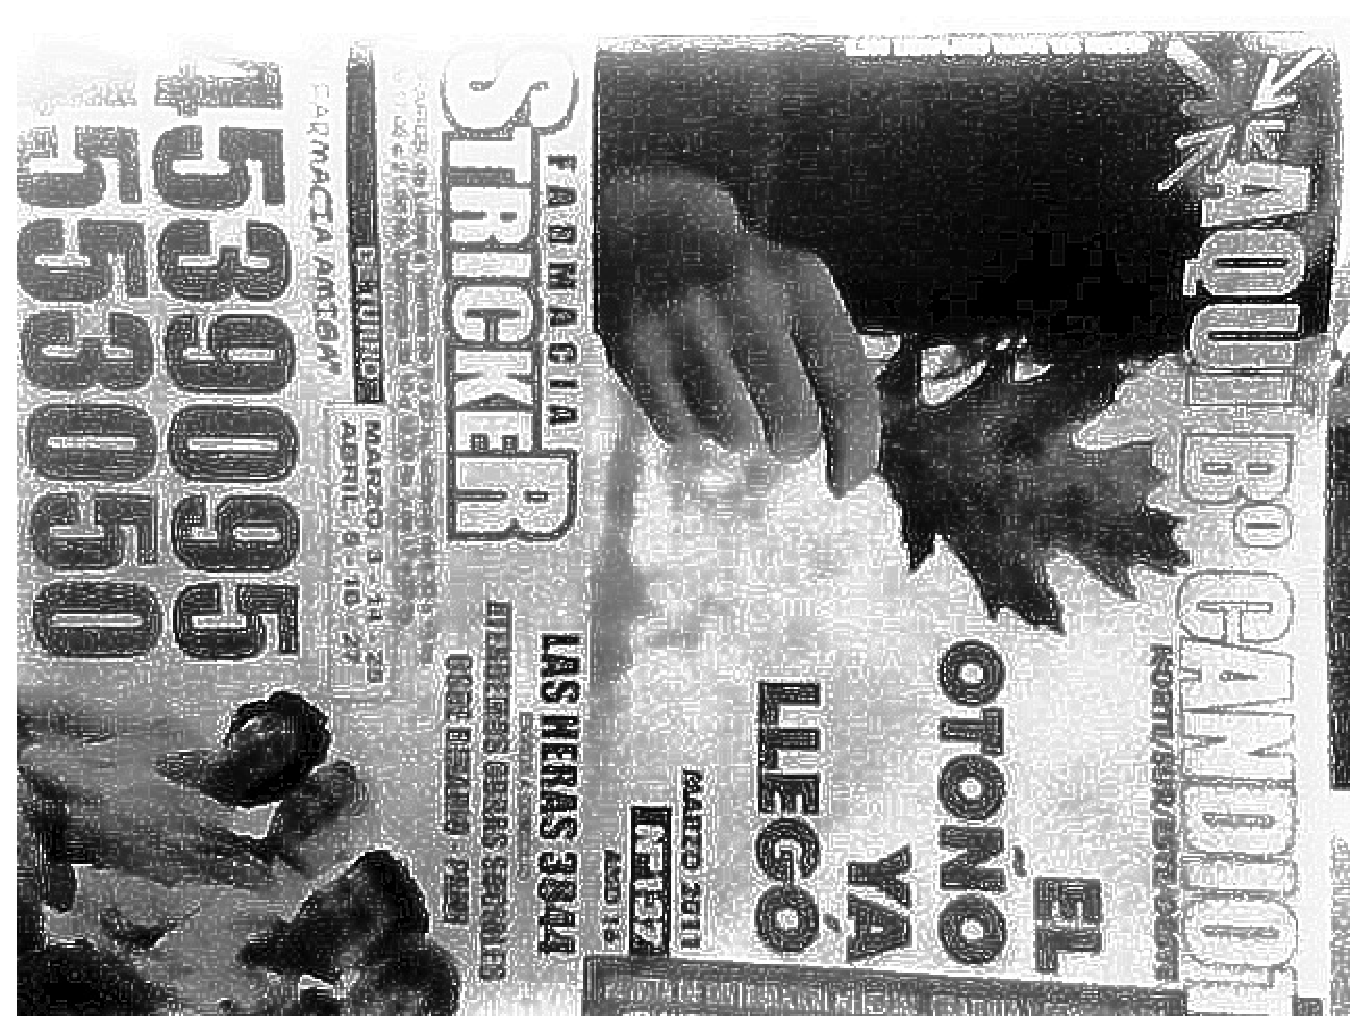
\includegraphics[width=0.32\textwidth]{../../exp1/train_normal_BN/keypoints5} \label{fig:iluminacion_BN_ecyaltapotencia}}\\
% %     \caption*[Resultados de aplicar las técnicas para la mejora en iluminación y detalles en condición $B_{N}$]{Resultados de aplicar las técnicas para la mejora en iluminación y detalles en condición $B_{N}$.}
%     \label{fig:mejoras_iluminacion_normal_BN}               %% Etiqueta para la figura entera
%   \end{figure}
% \end{frame}

% \begin{frame}{Condición $B_{H}$}
%     \begin{figure}
%       \centering
%       \subfloat[\tiny{Imagen patrón con Ilum. $B_{H}$}]{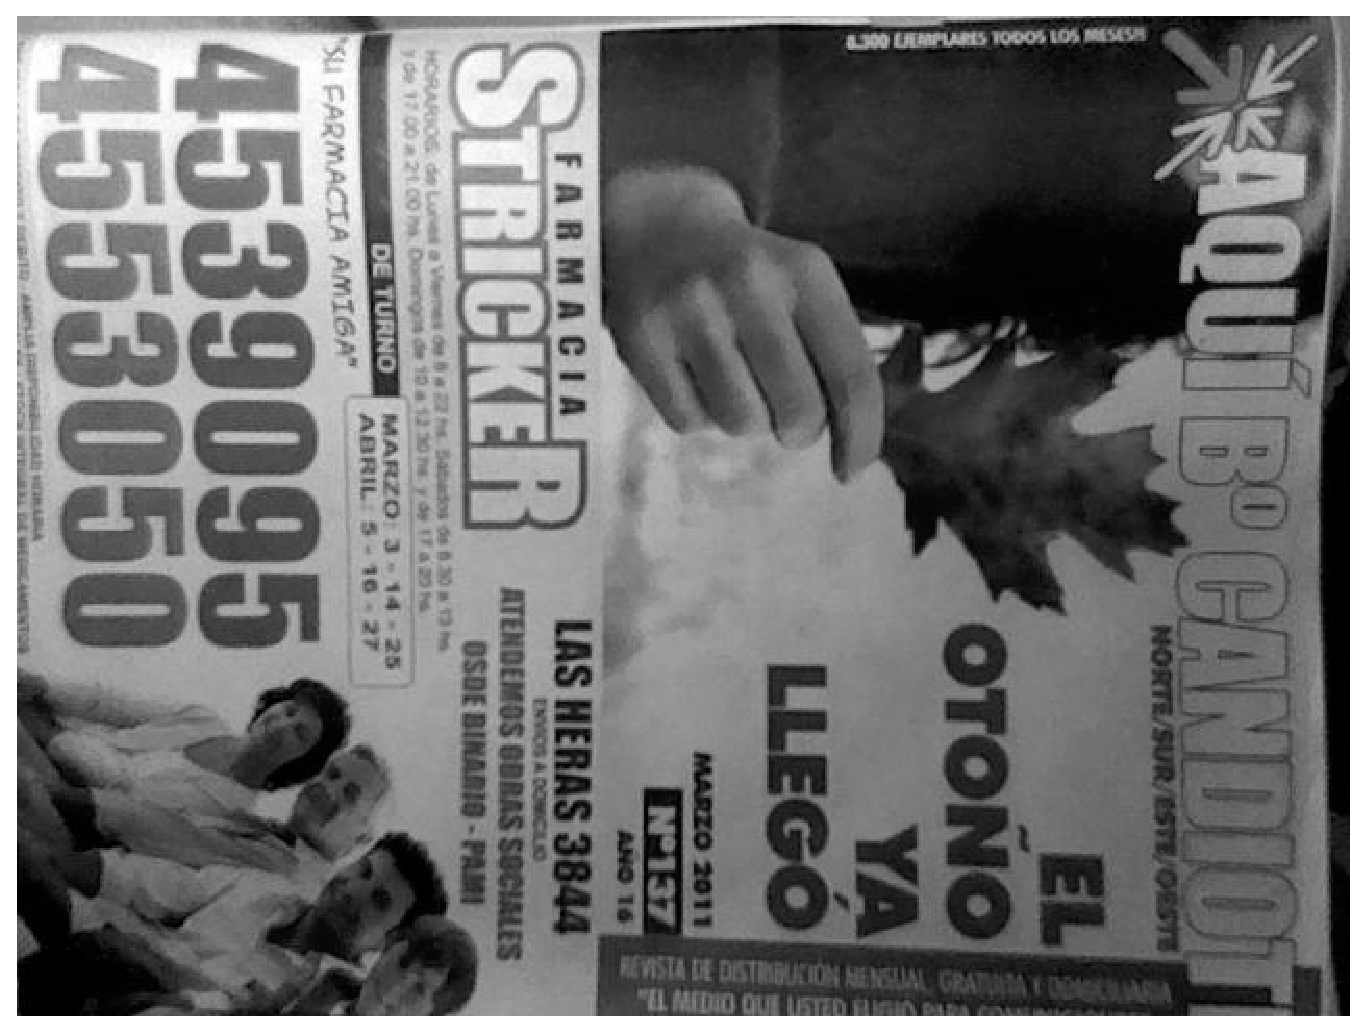
\includegraphics[width=0.32\textwidth]{../../exp1/train_brillante_BH/train_brillante_grises} \label{fig:iluminacion_BH_original}}
%       \subfloat[\tiny{Transformación logarítmica}]{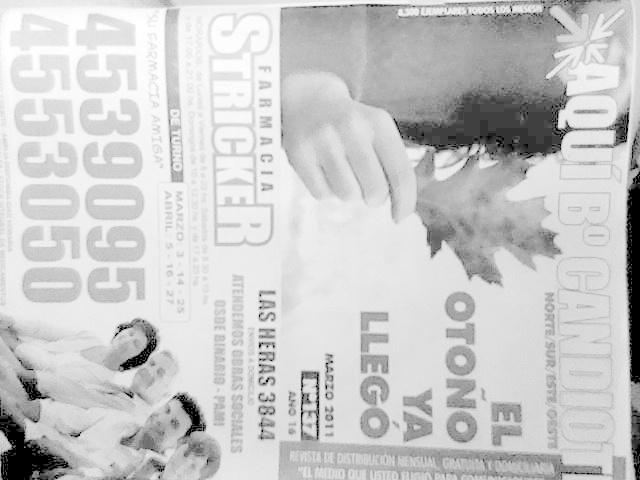
\includegraphics[width=0.32\textwidth]{../../exp1/train_brillante_BH/train_brillante622} \label{fig:iluminacion_BH_logaritmica}}
%       \subfloat[\tiny{Ecualización}]{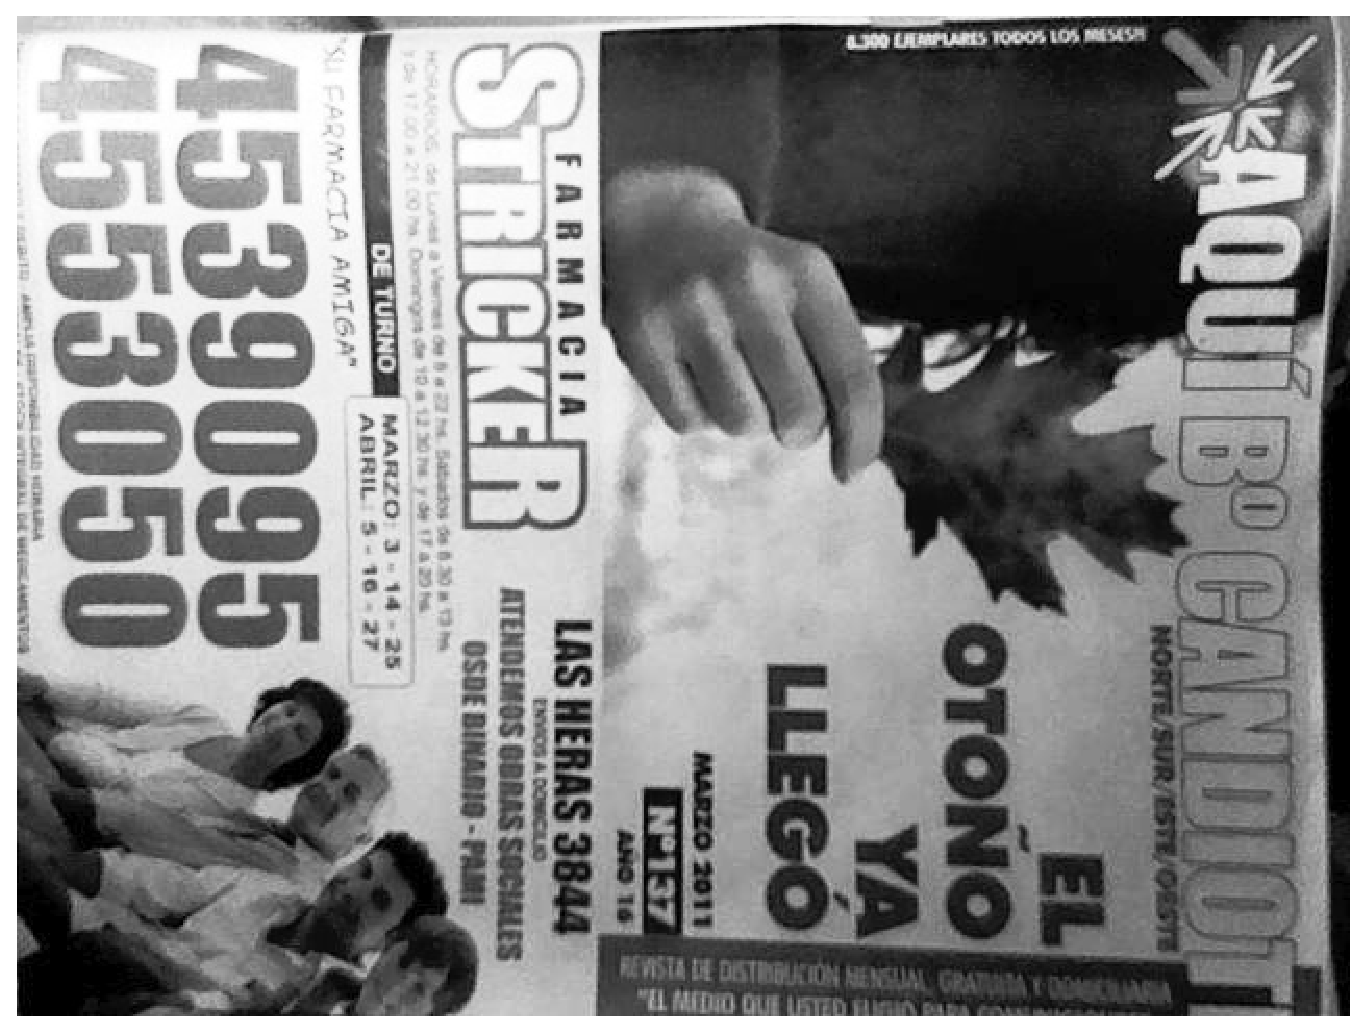
\includegraphics[width=0.32\textwidth]{../../exp1/train_brillante_BH/keypoints2} \label{fig:iluminacion_BH_ecualizacion}}\\
%       \subfloat[\tiny{Filtrado pasa altos}]{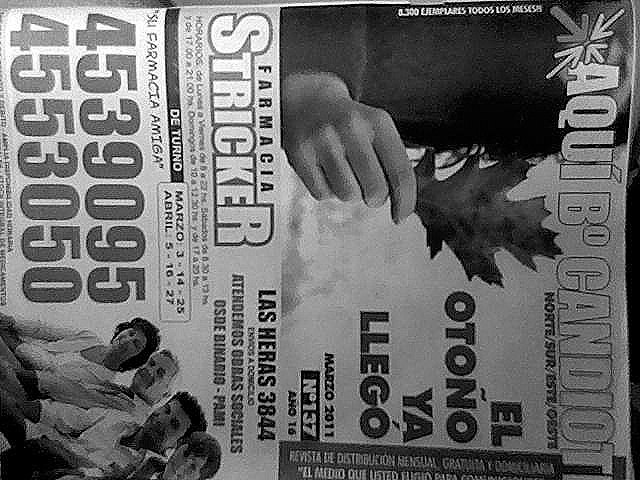
\includegraphics[width=0.32\textwidth]{../../exp1/train_brillante_BH/keypoints3} \label{fig:iluminacion_BH_pasaaltos}}
%       \subfloat[\tiny{Filtrado de alta potencia}]{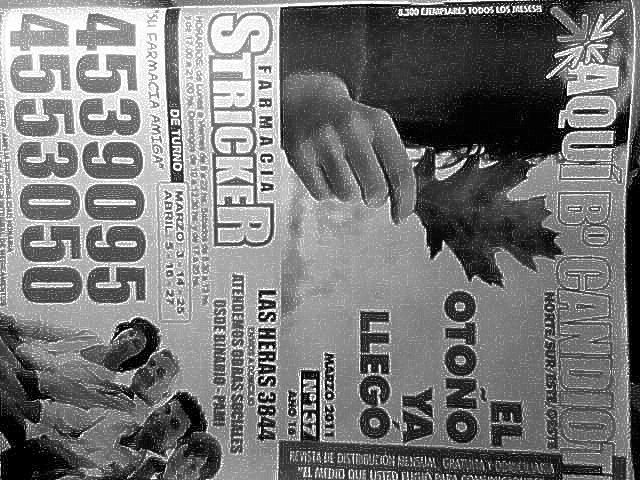
\includegraphics[width=0.32\textwidth]{../../exp1/train_brillante_BH/keypoints4} \label{fig:iluminacion_BH_altapotencia}}
%       \subfloat[\tiny{Ecualización + filtrado de alta potencia}]{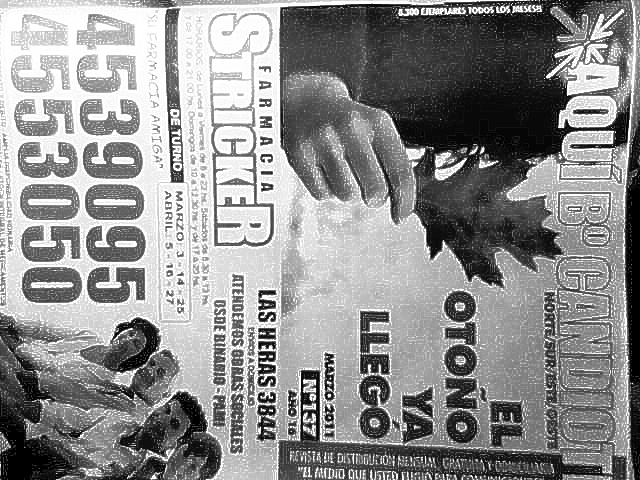
\includegraphics[width=0.32\textwidth]{../../exp1/train_brillante_BH/keypoints5} \label{fig:iluminacion_BH_ecyaltapotencia}}
% %       \caption*[Resultados de aplicar las técnicas para la mejora en iluminación y detalles en condición $B_{H}$]{Resultados de aplicar las técnicas para la mejora en iluminación y detalles en condición $B_{H}$}
%       \label{fig:mejoras_iluminacion_brillante_BH}               %% Etiqueta para la figura entera
%     \end{figure}
% \end{frame}

%%%%%%%%%%%%%%%%%%%%%%%%%%%%%%%%%%%%%%%%%%%%%%%%%%%%%%%%%%%%%%%%%%%%%%%%%%%%%%%%%%%%%%%%%%%%%%%%%%%
\begin{frame}{Condición $B_{L}$}
\note[item]{Mejores resultados para $B_{L}$ $\rightarrow$ \textit{ecualización}: Maximización del contraste y combinación de \textit{ecualización y filtrado de alta potencia}}
  \begin{figure}
  \centering
  \subfloat[\scriptsize{Imagen patrón con Ilum. $B_{L}$}]{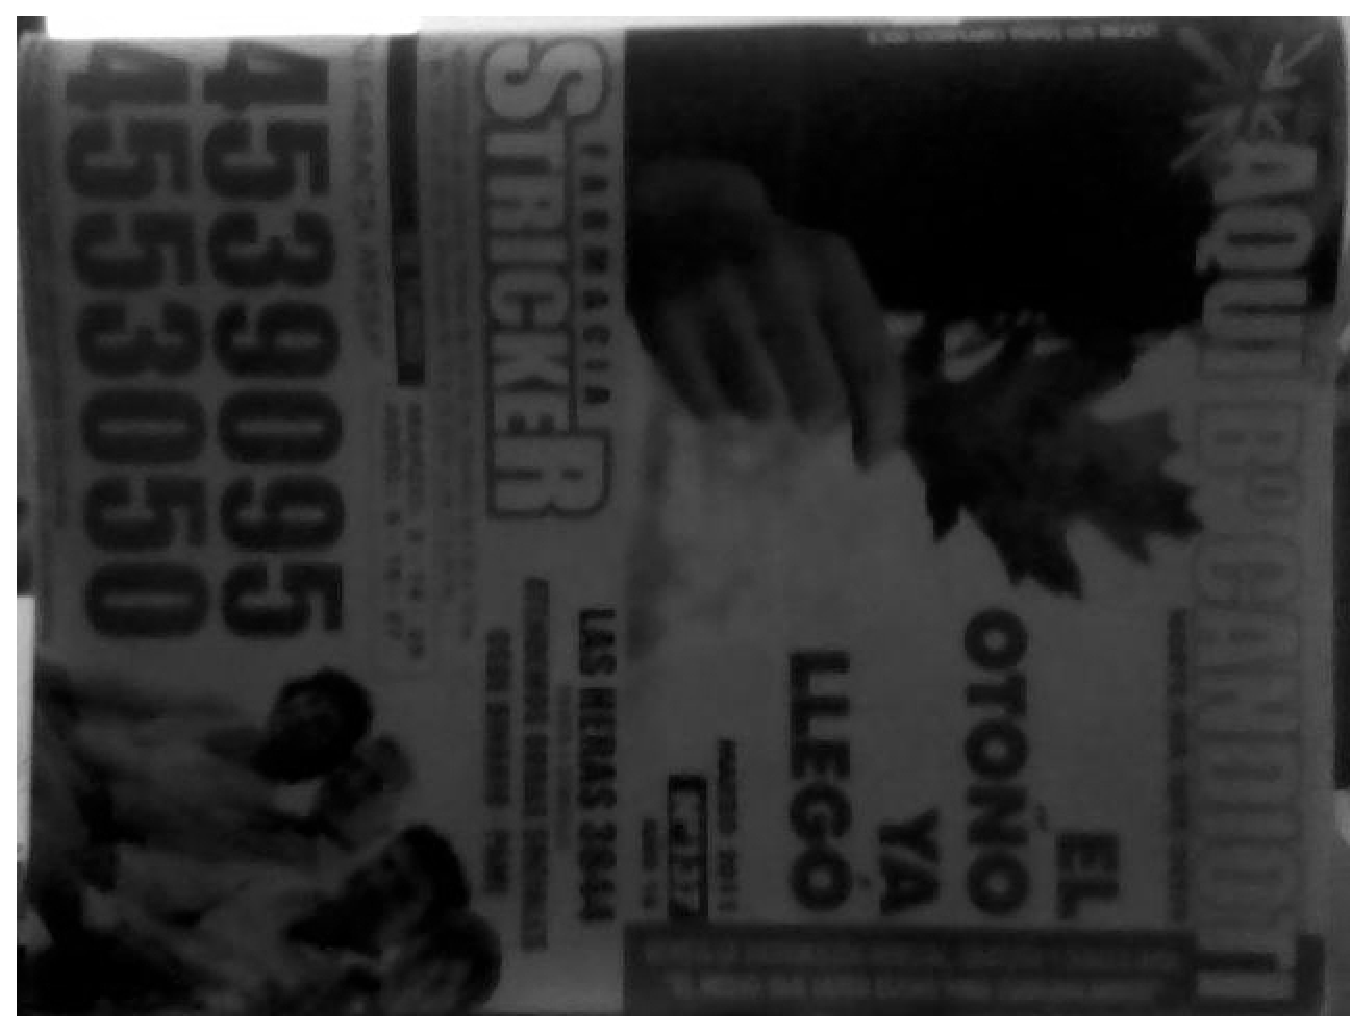
\includegraphics[width=0.32\textwidth]{../../exp1/train_oscura_BL/train_oscura_grises} \label{fig:iluminacion_BL_original}}
  \subfloat[\scriptsize{Transformación logarítmica}]{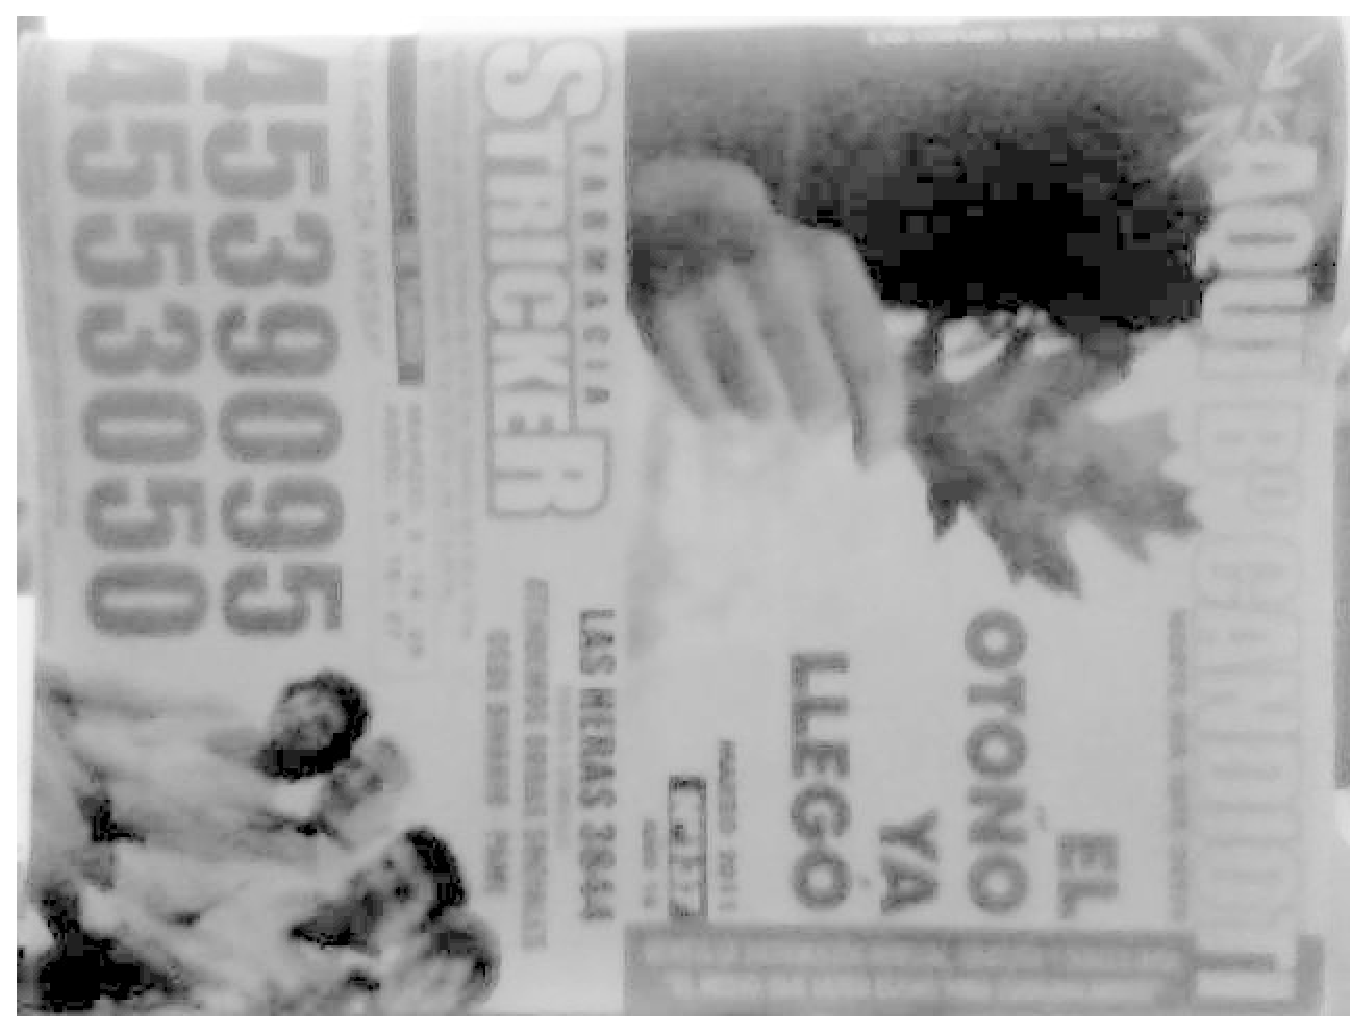
\includegraphics[width=0.32\textwidth]{../../exp1/train_oscura_BL/train_oscura453} \label{fig:iluminacion_BL_logaritmica}}
  \subfloat[\scriptsize{Ecualización}]{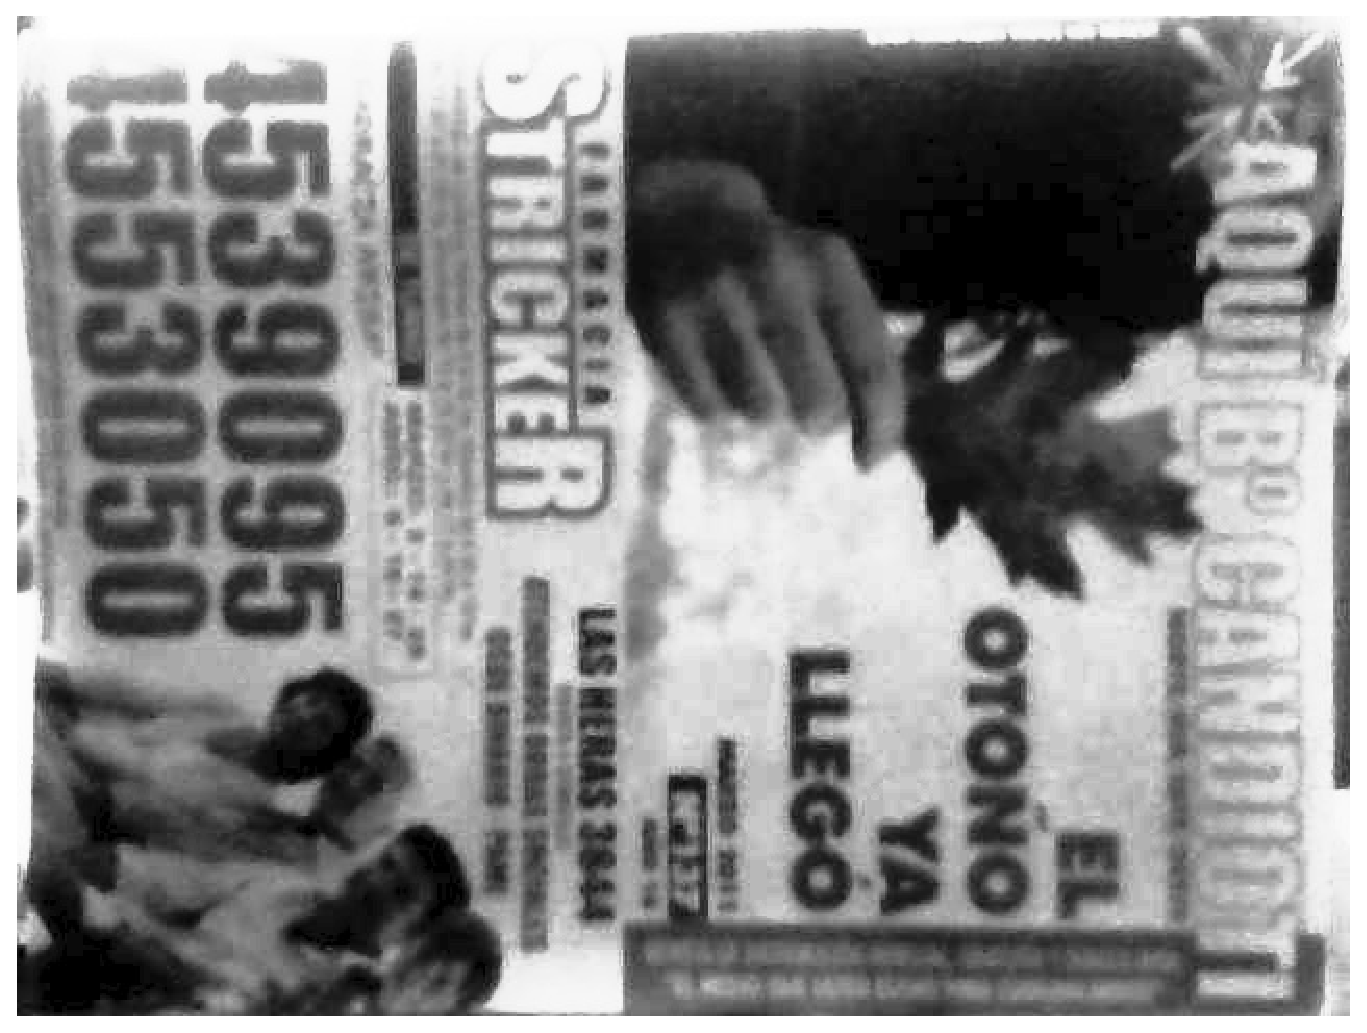
\includegraphics[width=0.32\textwidth]{../../exp1/train_oscura_BL/keypoints2} \label{fig:iluminacion_BL_ecualizacion}}\\
  \subfloat[\scriptsize{Filtrado pasa altos}]{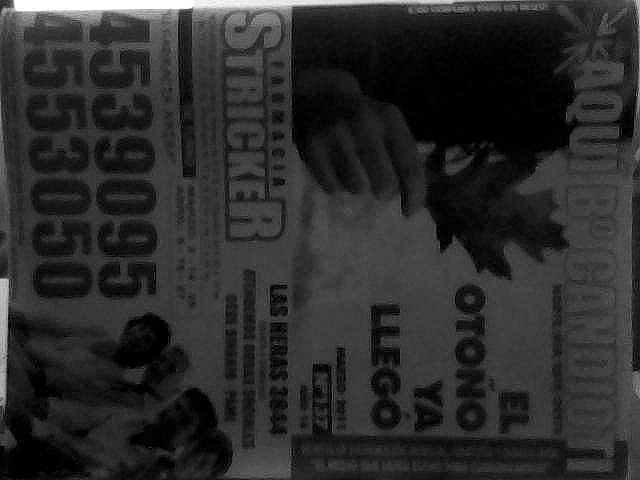
\includegraphics[width=0.32\textwidth]{../../exp1/train_oscura_BL/keypoints3} \label{fig:iluminacion_BL_pasaaltos}}
  \subfloat[\scriptsize{Filtrado de alta potencia}]{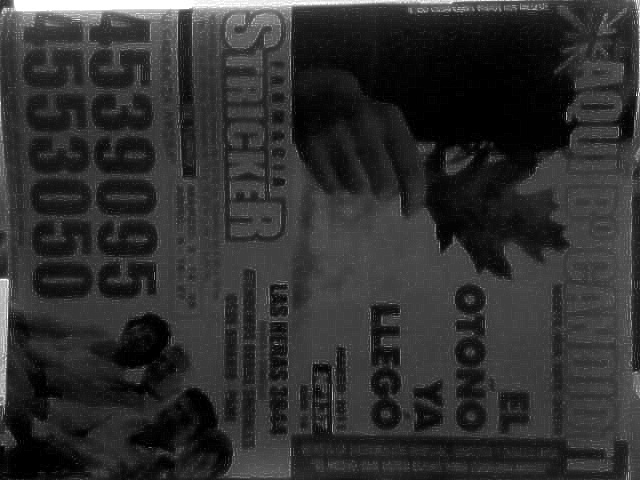
\includegraphics[width=0.32\textwidth]{../../exp1/train_oscura_BL/keypoints4} \label{fig:iluminacion_BL_altapotencia}}
  \subfloat[\scriptsize{Ecualización + filtrado de alta potencia}]{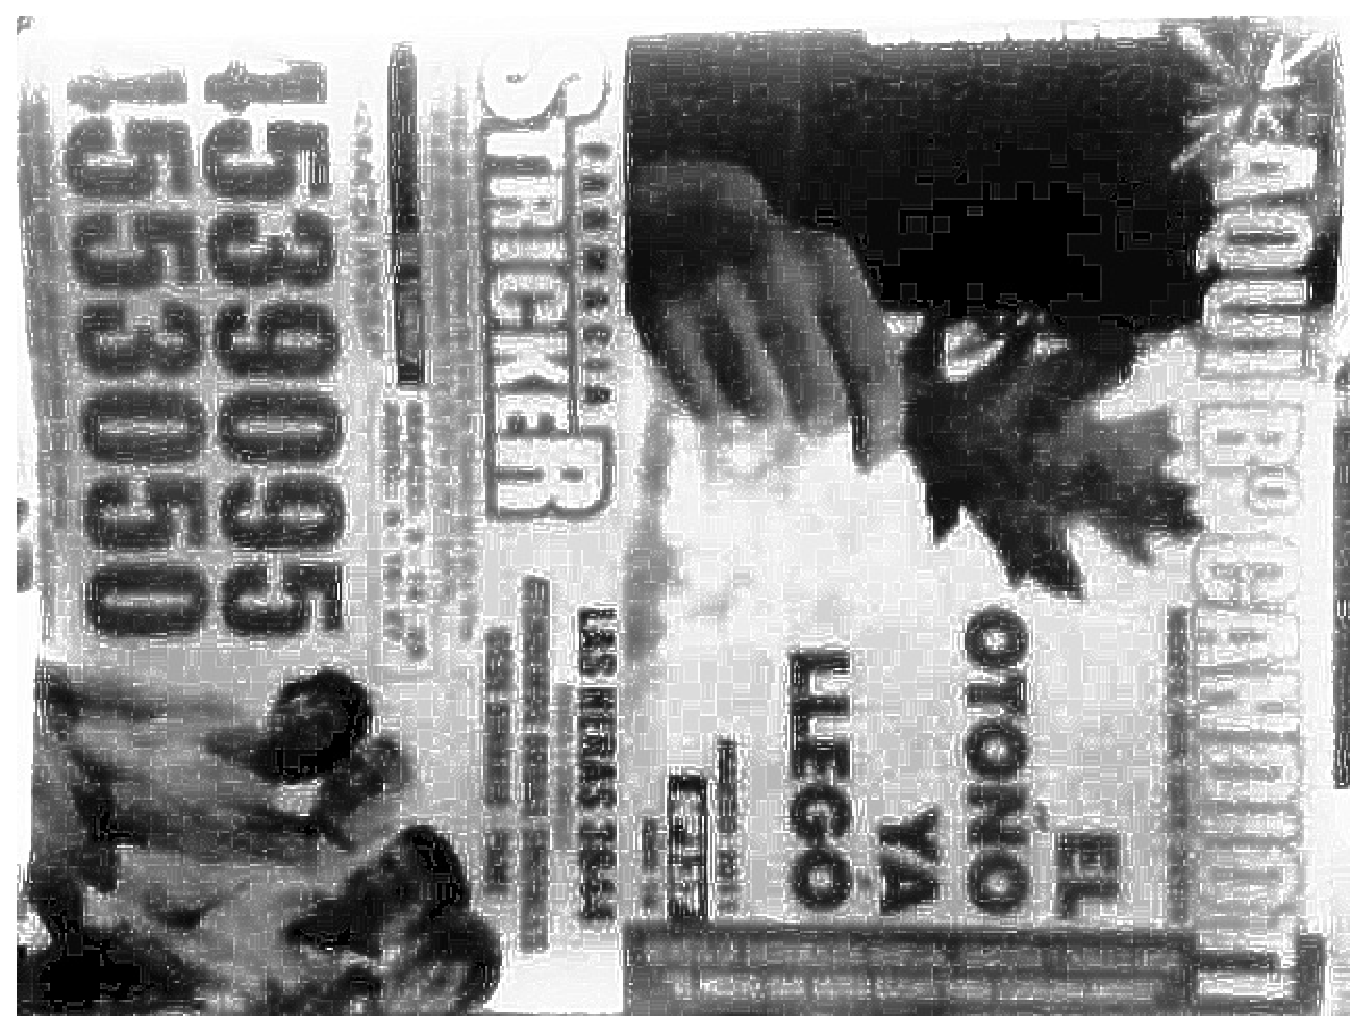
\includegraphics[width=0.32\textwidth]{../../exp1/train_oscura_BL/keypoints5} \label{fig:iluminacion_BL_ecyaltapotencia}}
%   \caption*[Resultados de aplicar las técnicas para la mejora en iluminación y detalles en condición $B_{L}$]{Resultados de aplicar las técnicas para la mejora en iluminación y detalles en condición $B_{L}$}
  \label{fig:mejoras_iluminacion_oscura_BL}               %% Etiqueta para la figura entera
  \end{figure}
\end{frame}

\begin{frame}{Tiempos y cantidad de características}
    Umbral hessiano: $700$ e igual para las tres condiciones de iluminación. 
	\note[item]{el umbral se estableció empíricamente}
    \begin{table}[htbp]
      \caption*{Tiempo de procesamiento en milisegundos y cantidad de características sobre la imagen patrón en condiciones de iluminación $B_{N}$, $B_{H}$ y $B_{L}$.}
	\begin{tabular}{|l|r|c|c|c|}
	  \hline
	  %& \multicolumn{2}{c|}{\textbf{Iluminación Normal}} \\ \hline
	  & \multicolumn{1}{c|}{\textbf{t [ms]}} & \textbf{$B_{N}$} & \textbf{$B_{H}$} & \textbf{$B_{L}$}\\ \hline
	  \textbf{Sin Proc} & 0,00 &  958 & 1297 & 154\\ \hline
	  \textbf{Logaritmo} & 7,15 & 702 & 950 & 83\\ \hline \note[item]{Tiempo del logaritmo superior, se cree que es por la forma en que fue implementado (openCV trae implementado el log neperiano  y no el en base 10. La compilación de la librería con Intel IPP podría mejorar. Como la cantidad de puntos característicos es menor (excepto cuando hay baja iluminación), no se le dio importancia.)}
	  \textbf{Ecualización} & \textbf{0,70} & 1546 & 1472 & 1233\\ \hline
	  \textbf{F. Pasa Altos} & 1,26 &  1633 & 2006 & 269\\ \hline
	  \textbf{F. Alta Pot.} & 3,10 & 1952 & 2216 & 353\\ \hline \note[item]{F. Pasa altos y alta potencia: Las técnicas que involucran una operación de convolución obtienen tiempos mayores que las demás}
	  \textbf{Ec.+F. Alta Pot.} & 4,31 & \textbf{2704} & \textbf{2443} & \textbf{2002}\\ \hline 
	\end{tabular}
	\note[item]{combinación de ec. y F. de alta potencia resulta mayor por ser la suma de las dos anteriores}
	\note[item]{Tiempos: $\textrm{Sin proc.}<\textrm{Ec.}<\textrm{F. P. Altos}<\textrm{F. Alta pot.}<\textrm{Ec.+F. Alta Pot}<\textrm{log}$}
      \label{tabla:tiempos_realce_iluminacion}
    \end{table}    
\end{frame}

\begin{frame}{Cantidad de características}
% En el gráfico de la Fig. \ref{graph:comparacion_cantptos} se presenta una comparación de la cantidad de puntos detectados para las condiciones $B_{N}$, $B_{H}$ y$B_{L}$ establecidas. Claramente se advierte que cuando se realiza la combinación de \textit{ecualización y filtrado de alta potencia} en el caso de un ambiente en condición $B_{N}$, la cantidad de puntos detectados casi llega a triplicarse, respecto de cuando no se aplica técnica alguna. En tanto que en una condición $B_{H}$, la detección se duplica. Si analizamos lo que pasa en la condición de iluminación $B_{L}$, la cantidad de características posee valores bajos respecto de las otras condiciones de iluminación, ésta diferencia se evidencia aún más cuando no se aplica la ecualización, ya que los \textit{filtros pasa altos y de alta potencia} actúan sobre una imagen oscura sobre la que realzan los detalles, pero la diferencia de grises entre píxeles vecinos resulta insuficiente para una correcta detección.
  \note[item]{Marcelo: Explicar bien el gráfico que es lo que se ve y observa. Cuanto más largas las barras mejor es. En todos los casos se mejora y queda a criterio del usuario usar una u otra. NO EXPLICAR EL LOGARITMO}
  \note[item]{Marcelo: no se entendió la gráfica de tiempos, nombrarla mejor!}
  \begin{figure}[tbhp]
   \centering
        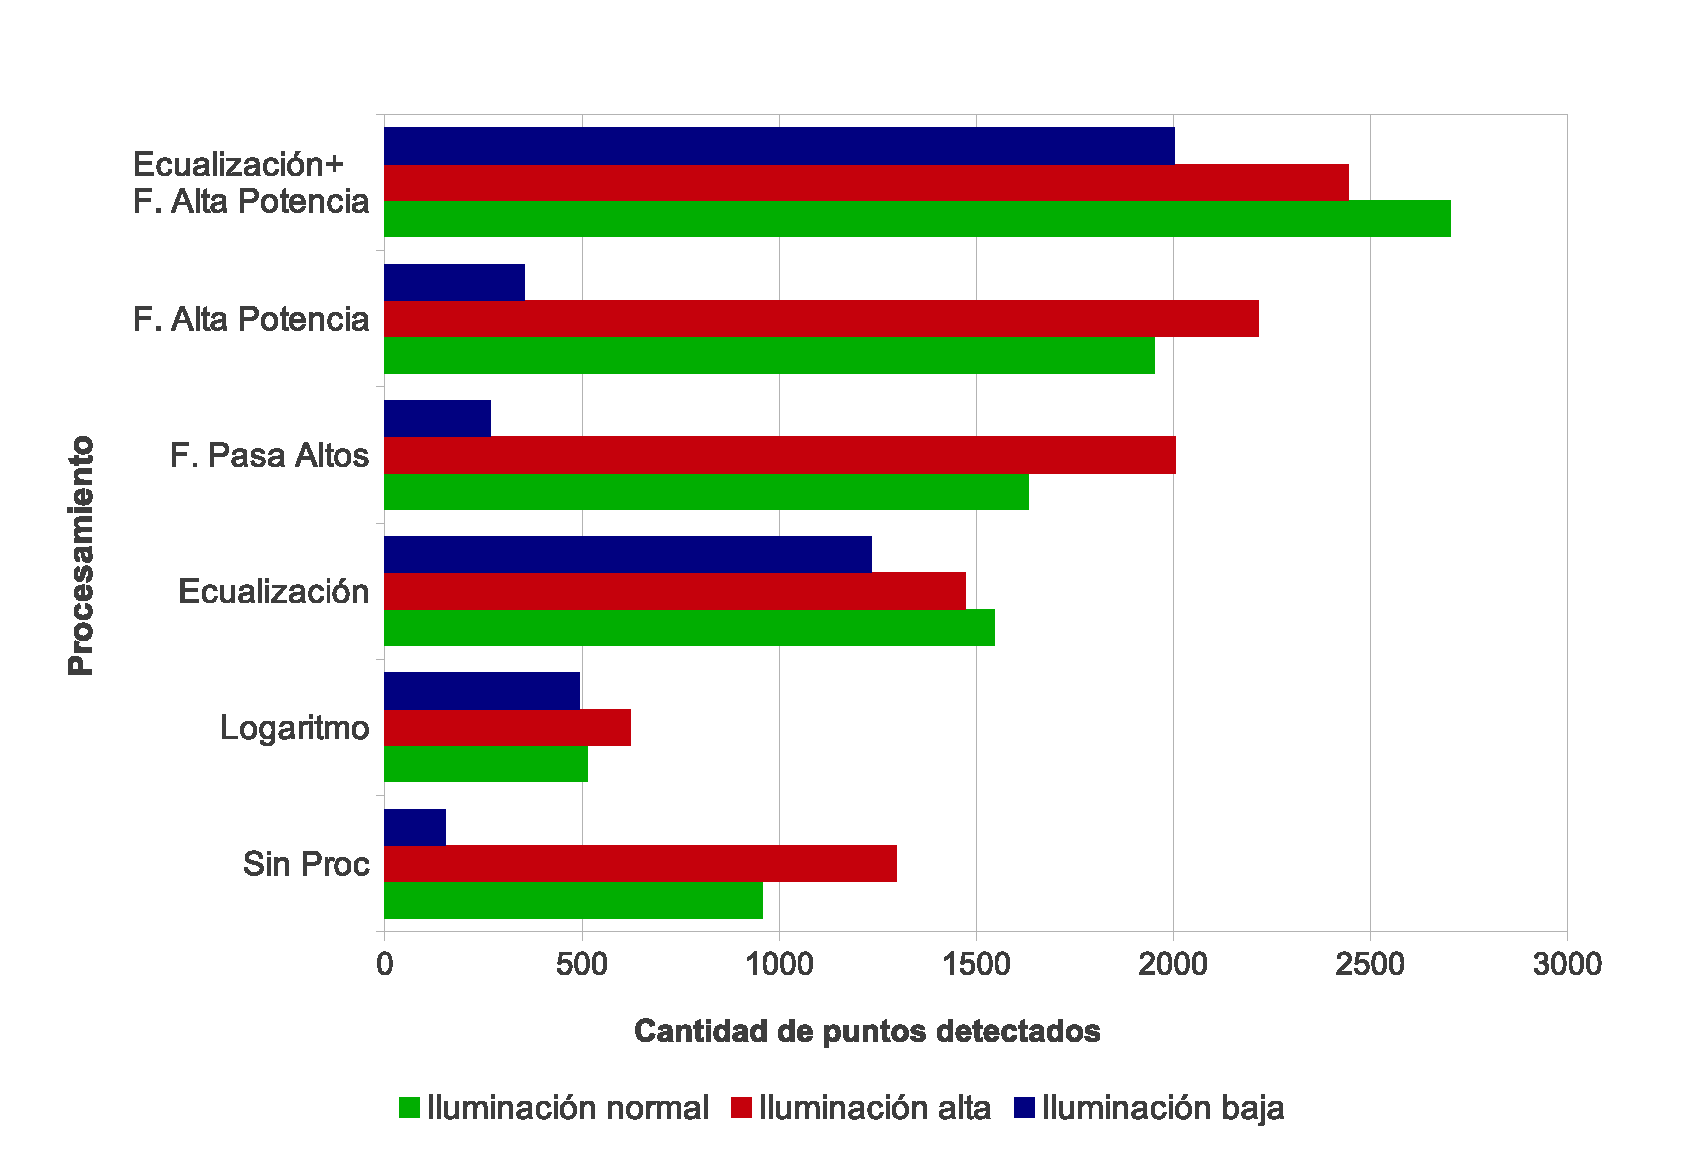
\includegraphics[scale=0.38]{../../pruebas_modif/graph_ptos_realces_presentacion1}
%     \caption*{\tiny{Cantidad de puntos detectados para la imagen con luminosidad normal (Fig. \ref{fig:train_normal}), alta (Fig. \ref{fig:train_brillante}) y baja (Fig. \ref{fig:train_oscura}).}}
   \label{graph:comparacion_cantptos}
  \end{figure}
   \note[item]{En $B_{N}$, la Ec.+filtrado de Alta Pot. la cant. de puntos se triplica. En $B_{H}$ se duplica respecto de Sin Proc.}
   \note[item]{Cant. de caract. detectadas $B_{N}$ y $B_{H}$: $\textrm{Log.}<\textrm{Sin proc.}<\textrm{Ec.}<\textrm{F.P altos}<\textrm{F.A.potencia}<\textrm{Ec.+F.A.potencia}$}
   \note[item]{Cant. de caract. detectadas $B_{L}$: $\textrm{Sin proc.}<\textrm{F.P altos}<\textrm{F.A.potencia}<\textrm{Log.}<\textrm{Ec.}<\textrm{Ec.+F.A.potencia}$}
   \note[item]{Combinacion de ec y filtro de alta pot, es la que mayor cantidad de detecciones de puntos presenta, producto de una iluminación más uniforme y luego el realce de los detalles.}
   \note[item]{Pasa altos y alta potencia realzan las altas frecuencias y discontinuidades. Alta potencia detecta más que el pasa altos porque no afecta las bajas frecuencias.}
   \note[item]{ecualización se obtienen más puntos que sin procesamiento, puede considerarse útil si la prioridad es el tiempo}
   \note[item]{Log solo incrementa puntos en la imagen con condición de iluminación baja. En condiciones de iluminación normal y alta el Log detecta menos características porque poseen intensidades más homogéneas y por lo tanto menor distinción en los detalles. En baja iluminación se incrementa como consecuencia de la expansión del rango dinámico}
\end{frame}

\begin{frame}{Experimento 1: conclusiones}
  \begin{itemize}
   \item En condiciones $B_{N}$ y $B_{H}$ resultados aceptables sin pre-procesamiento de iluminación o realce de detalles.
      \note[item]{Aplicar las técnicas que aumentan la cantidad de características, mejora la cantidad de características pero repercuten en el tiempo de procesamiento}
   \item Aplicar técnicas repercute negativamente en el tiempo de procesamiento pero aumenta la cantidad de puntos detectados.
   \item Determinar técnicas a utilizar y umbral hessiano:
      \begin{itemize}
	\item ¿Qué se desea priorizar: calidad en la detección o velocidad de ejecución?
	\item ¿Cuáles son las condiciones del ambiente? \note[item]{condiciones de iluminación}
      \end{itemize}
   \end{itemize}
\end{frame}

\begin{frame}{Experimento 1: conclusiones}
Prueba en condición de iluminación baja ($B_{L}$).
 \begin{itemize}
    \item En la práctica se presentan casos de detección ``intermitente'' o nula en condición $B_{L}$.
%       \begin{itemize}
% 	\item 
% 	\item condiciones intermedia entre $B_{L}$ y $B_{N}$
%       \end{itemize}
      \note[item]{Obtener mayor cantidad de características no presenta garantías de lograr una mejor detección (existencia de posibles características espurias)(*). SIN EMBARGO!}
  \end{itemize}
   
  \begin{itemize}
    \item La ecualización o ecualización+filtro de alta potencia mejoran la detección.
    \item Aumentar la cantidad de características produce una mejora en la detección. 
	\note[item]{Aumentar en el sentido de aplicar un realce de iluminación y no  de variar el umbral hessiano.}
    \item Una variación del umbral no produce resultados significativamente mejores. 
	\note[item]{No alcanza a detectar las características por ser muy oscura la imagen. Esto no tiene que ver con el umbral hessiano.}
  \end{itemize}
\end{frame}

\subsubsection*{}
\begin{frame}{Experimento 2}
\note[item]{Marcelo: no decir estables! sino que se quería obtener conclusiones en los ambientes donde el método es probable que sea ejecutado en condiciones de iluminación normal y alta}
\begin{block}{Experimento 2: costo computacional del método propuesto}
 Evaluación detallada del costo computacional en etapa de ejecución, considerando los pasos del algoritmo propuesto.
\end{block}
 \begin{itemize}
  \item Tiempos que insumen los procesos del método.
  \note[item]{Condicionales del método que permiten mejorar la detección y minimizar los tiempos de procesamiento}
  \item 2 pruebas en condiciones de iluminación $B_{N}$ y $B_{H}$. \note[item]{no se usa $B_{L}$ por efecto de ``parapadeo'' y se desean obtener conclusiones cuando la detección resulta estable}
  \item Sin técnicas de ``Pre-Procesamiento de iluminación y realce de detalles''. \note[item]{se dejan a criterio del usuario y para las condiciones de iluminación dadas no fue necesario aplicarlas}
  \note[item]{Marcelo: Decir bien ``Pre procesamiento de iluminación y realce de detalles''}
 \end{itemize}
\end{frame}
 
 \begin{frame}{Pruebas}
 \note[item]{Marcelo: Se hicieron pruebas para 2 videos sobre el flujo de video}
 \note[item]{Se realizaron 2 pruebas}
      \begin{block}{Prueba 1 (P1)}
	  \begin{itemize}
	    \item Duración: 1:50 minutos.
	    \item Umbral hessiano: 3500.
	    \item Imagen con condición $B_{N}$.% \ref{fig:train_normal} \footnote{Video de la prueba: \url{http://youtu.be/E8uGptzdEiw}}
	  \end{itemize}
      \end{block}

      \begin{block}{Prueba 2 (P2)}
	  \begin{itemize}
	    \item Duración: 1:35 minutos.
	    \item Umbral hessiano: 5000.
	    \item Imagen con condición $B_{H}.$% \ref{fig:train_brillante} \footnote{Video de la prueba: \url{http://youtu.be/Pkiub9ZXP4k}}
	  \end{itemize}
	  \note[item]{por cuestiones de brevedad se presenta la p1 solamente ya que con esta se obtuvieron resultados similares}
      \end{block}
\end{frame}

% \begin{frame}{Datos computados}
%   \begin{itemize}\small{
%     \item Tiempo de \textit{detección de movimiento},
%     \item Tiempo de \textit{extracción y descripción de las características en BR} *,
%     \item Tiempo de \textit{búsqueda de correspondencias} *,
%     \item Tiempo de \textit{estimación de la homografía} *,
%     \item Tiempo de comprobación \textit{contorno convexo y vértices válidos} *,
%     \item Tiempo de \textit{transformación perspectiva de la imagen de RA utilizando la homografía} *,
%     \item Cuadros por segundo (FPS),
%     \item Total de puntos detectados en la imagen patrón,
%     \item Total de puntos detectados en la imagen objeto,
%     \item Total de coincidencias potencialmente válidas.
%   }
%   \end{itemize}
% \end{frame}

% \begin{frame}{Análisis de 2 procesos}
%     \begin{block}{``Proceso con bifuración en condicionales (\textbf{PCBC})''}
% 	Las operaciones marcadas con (*) pueden ignorarse en el ciclo de ejecución sin impedir que se realice el enriquecimiento de la realidad.
% 	  \note[item]{Las operaciones marcadas con (*) pueden ignorarse.}
% 	  \note[item]{SI la comprobación de contornos convexos y vértices válidos (CCVV) no se cumple, entonces no se calcula la Transformación Perspectiva(TP)}
% 	  \note[item]{si la homografía no es detectada, no se realiza la CCCV y por ende tampoco la TP}
% 	  \note[item]{si no se detecta movimeinto en la escena, ninguno de los procesos es ejecutado}
% 	  \note[item]{Todos estos condicionales produce que el tiempo rpomedio de procesamiento disminuya cuando alguna o todas las operaciones son ignoradas}
%     \end{block}
%     \begin{block}{``Proceso sin bifuración en condicionales (\textbf{PSBC})''}
%     \end{block}
% \end{frame}

\begin{frame}{Tiempos de operación de procesos en P1}
  \note[item]{Marcelo: Aclarar que cuanto menor son las barras mejor es el método}
  \note[item]{Marcelo: Aclarar que existe un método estándar en donde los condicionales no están y el método propuesto por nosotros.}
  \begin{figure}[tbhp]
   \centering
        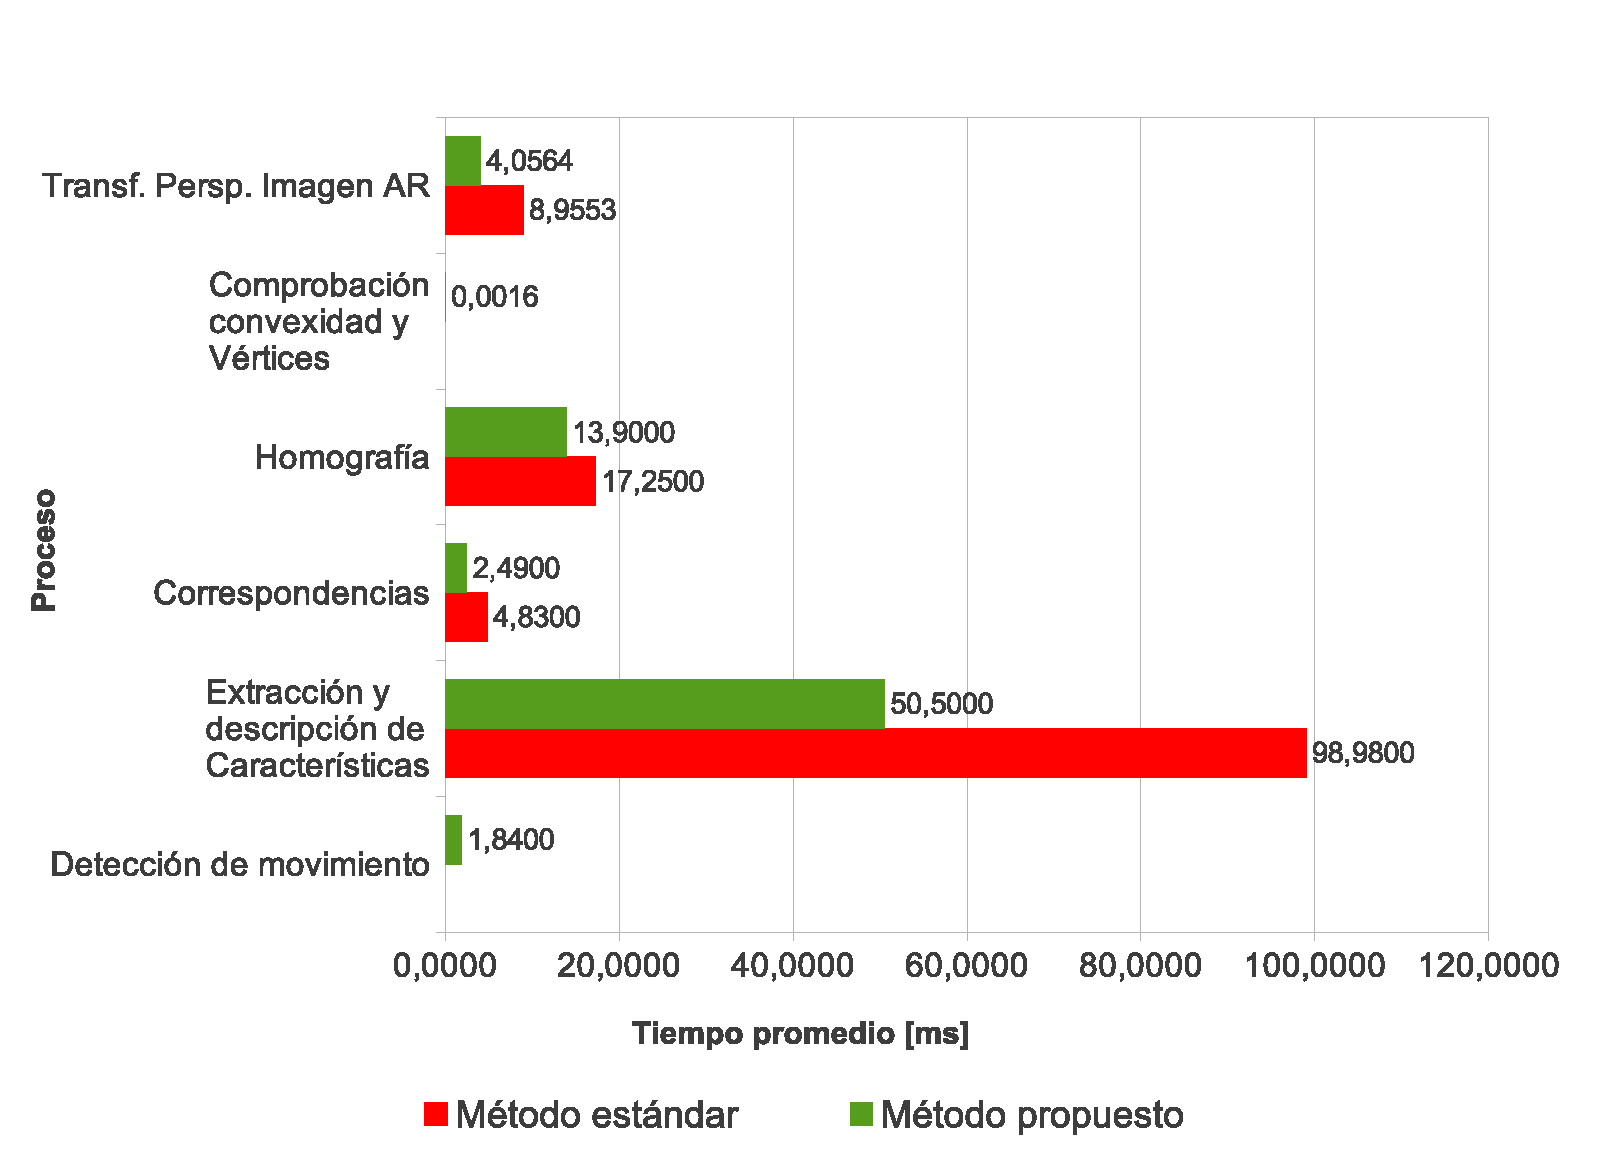
\includegraphics[scale=0.38]{../../pruebas_modif/3500_sinproc/graph_tiempos_3500_presentacion1}
    \caption*{\tiny{Tiempos promedios de operación por procesos en la prueba 1}}
   \label{graph:graph_tiempos_3500}
  \end{figure}
  \note[item]{+comprobación de área BR, y luego actuación del buffer (condición de presencia previa => mejoran aún más)}
  \note[item]{Tiempos promedios en la fase de ejecución de P1 para el método estándar y el propuesto.}
  \note[item]{Proceso de extracción y descripción de características es el que más tiempo consume a pesar de realizarse en BR: \begin{itemize}
	\item Si BR = 50\% de la imagen patrón de $640 \times 480$ píxeles $\rightarrow$ representa un 42\% del tiempo para procesar toda la imagen
      \end{itemize}
  }
  \note[item]{Segundo aparece la estimación de la homografía por tratarse de un método iterativo que estima la matriz H y refina las coincidencias}
  \note[item]{Tercero queda la transofmración perspectiva que involucra una interpolación}
  \note[item]{Sigue la búsqueda de correspondencias (recordar que es aproximada y se utilizó randomized kdtrees)}
  \note[item]{sigue la detección de movimiento y la CCVV que están compuestas de operaciones triviales}
\end{frame}
% 
% \begin{frame}{P1}
% 
% \end{frame}

\begin{frame}{Conclusiones P1}
% tiempos en los diferentes procesos
%  \begin{itemize}
%   \item extracción y descripción de características es la que más tiempo requiere (a pesar de que se minimizó el procesamiento en un área de la imagen (BR)). Si el área BR en el que se extraen características es del 50\% de la imagen patrón en $B_{N}$} el tiempo de procesamiento representa un 42\% del tiempo total que se requería para extraer las características en la totalidad de la imagen.
%   \item segundo proceso que más tiempo consume es la estimación de la homografía por tratarse de un método iterativo que estima la matriz $H$ y refina las coincidencias
%   \item transformación perspectiva en tercer lugar por involucrar una interpolación,
%   \item les siguen búsqueda de correspondencias, la detección de movimiento y finalmente, la CCVV que está compuesta de operaciones triviales
%  \end{itemize}

%  total de puntos detectados y las potenciales correspondencias válidas
  \begin{block}{Objetivas}
      Tiempos:
      \begin{itemize}
	  \item Método estándar: $6.93$ FPS promedio.
	  \item Método propuesto: $28.35$ FPS promedio.
      \end{itemize}
  \end{block}
  
  \begin{block}{Subjetivas}
      \begin{itemize}
	  \item Eliminación de transformaciones fallidas.
	  \item Reducción de detecciones intermitentes.
	    \note[item]{Marcelo: El objeto virtual se sigue dibujando si se pierde en un frame. si pasa más de 3 frames perdidos, se deja de dibujar}
	    \note[item]{Marcelo: Ver si no me falta alguna conclusión más?}
	  \item Mayor fluidez en la reproducción. \note[item]{Naturalidad}
      \end{itemize}
  \end{block}
 %   \item segundo proceso que más tiempo consume es la estimación de la homografía por tratarse de un método iterativo que estima la matriz $H$ y refina las coincidencias
%   \item transformación perspectiva en tercer lugar por involucrar una interpolación,
%   \item les siguen búsqueda de correspondencias, la detección de movimiento y finalmente, la CCVV que está compuesta de operaciones triviales
%  
%  \begin{exampleblock}{Puntos y coincidencias}
%     \begin{itemize}
% 	\item 192 puntos claves en la imagen patrón
% 	\item en promedio 130 puntos en la imagen del flujo de video
% 	\item en promedio 38 pares de coincidencias potencialmente válidas (máximo de 81 pares)
%     \end{itemize}
%  \end{exampleblock}
\end{frame}

\begin{frame}{Imágenes prueba 1}
%   Umbral hessiano 3500 y la escena se encuentra en condición $B_{N}$ de iluminación.
    \note[item]{Marcelo: Explicar oclusión: en la quinta imagen se puede ver los dedos que están sobre el objeto a detectar y sin embargo se sigue viendo}
    \note[item]{Marcelo: Si la oclusión es por menos de 3 frames sigue funcionando}
    \begin{figure}[tbhp]
    \centering
    \subfloat{
\includegraphics[width=0.34\textwidth]{../../pruebas_modif/capturas/usables/train_normal} \label{fig:imagen_patron_ejemplo}}
    \subfloat{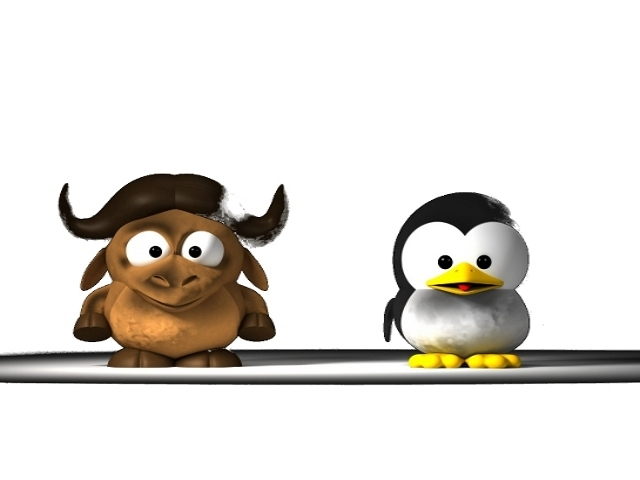
\includegraphics[width=0.34\textwidth]{../../pruebas_modif/capturas/usables/pinguino} \label{fig:imagen_objetoar_ejemplo}}
    \subfloat{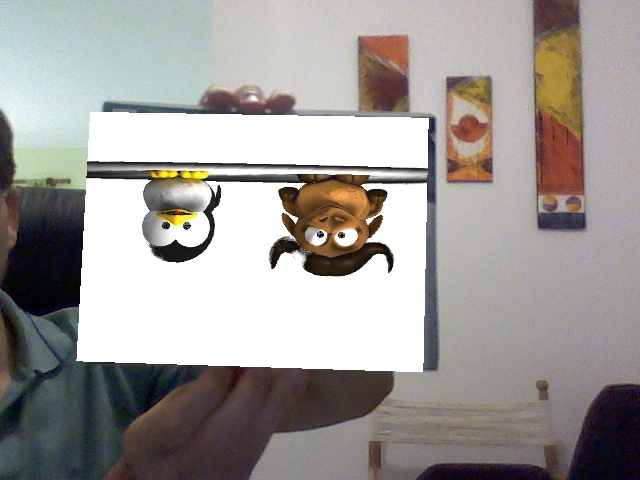
\includegraphics[width=0.34\textwidth]{../../pruebas_modif/capturas/usables/captured154} \label{fig:imagen_secuencia1_ejemplo}}\\
    \subfloat{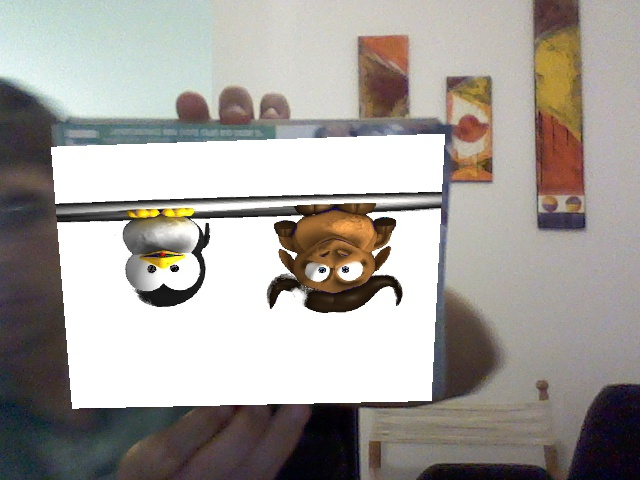
\includegraphics[width=0.34\textwidth]{../../pruebas_modif/capturas/usables/captured135} \label{fig:imagen_secuencia2_ejemplo}}
    \subfloat{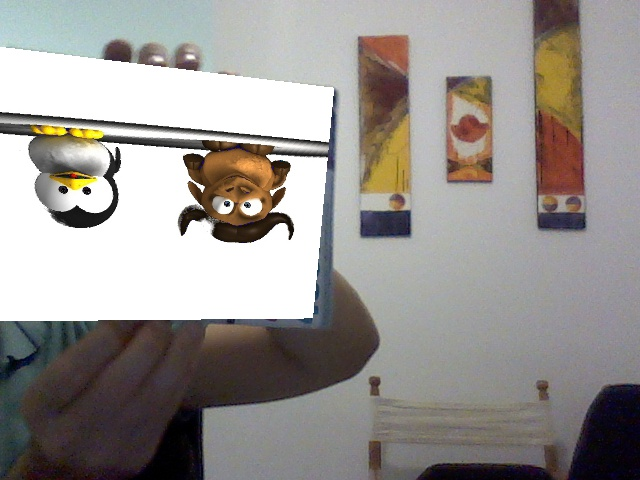
\includegraphics[width=0.34\textwidth]{../../pruebas_modif/capturas/usables/captured141} \label{fig:imagen_secuencia3_ejemplo}}
    \subfloat{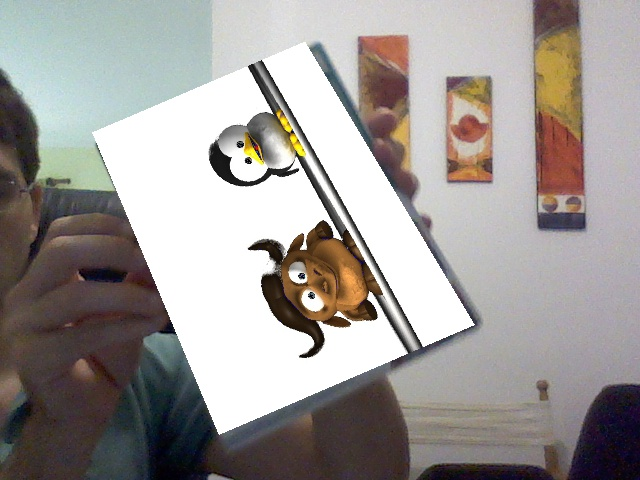
\includegraphics[width=0.34\textwidth]{../../pruebas_modif/capturas/usables/captured207} \label{fig:imagen_secuencia4_ejemplo}}
    \caption*{\tiny{Imagen patrón, objeto de RA y secuencia de imágenes (no sucesivas) con enriquecimiento de la realidad.}}
    \label{fig:secuencia_ejemplo_BN}               %% Etiqueta para la figura entera
    \end{figure}
\end{frame}

% \begin{frame}{Prueba 2}
%   \begin{itemize}
%     \item En $P2$ resultados similares a $P1$
%     \item La cantidad de puntos detectados en la imagen patrón $\uparrow$ a pesar de $\uparrow$ el umbral hessiano $\rightarrow$
%     La imagen sobre la cual se aplicó poseía mayor luminosidad y, por lo tanto mayores detalles apreciables.
%   \end{itemize}
% \end{frame}
%%%%%%%%%%%%%%%%%%%%%%%%%%%%%%%%%%%%%%%%%%%%%%%%%%%%%%%%%%%%%%%%%%%%%%%%%%%%%%%%%%%%%%%%%%%%%%%%%%%%%%%%%%%%%%%%%%%%%%%%%%%%%%%%%%%%%%%%%%%%%%%%%%%%
\subsection{Implementación de prototipos}
  \begin{frame}{Prototipos}
    \begin{itemize}
      \item Se enriquece la realidad mediante una imagen sobre la tapa de una revista.
	  \note[item]{algunos de estos ejemplos los hemos visto en las imágenes a lo largo de la presentación}
      \item Proveer información inherente a un producto comestible de forma publicitaria: video en condición $B_{N}$.
	\note[item]{se mostrará un video al finalizar la presentacion}%\url{http://youtu.be/j1xPZkglJHs}. 
    \end{itemize}
  \end{frame}

  \begin{frame}{Prototipo publicitario}
    \begin{figure}
	\centering
	\subfloat{
\includegraphics[width=0.33\textwidth]{../../imgvitina/vitina}\label{fig:prototipo_img_detect}}
	\subfloat{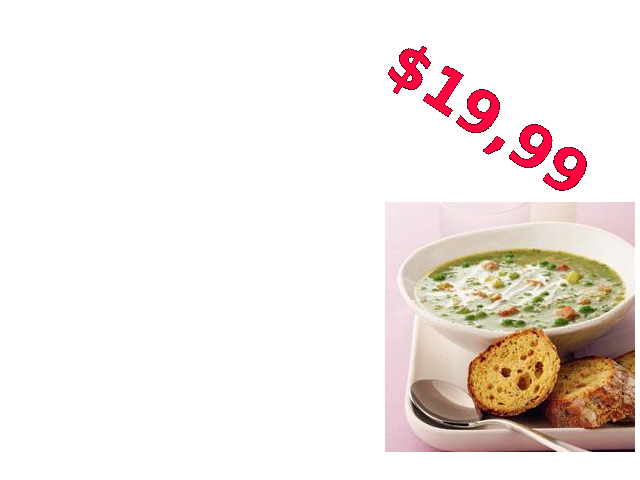
\includegraphics[width=0.33\textwidth]{../../imgvitina/preciosvirtuales}\label{fig:protitpo_img_ar}}
	\subfloat{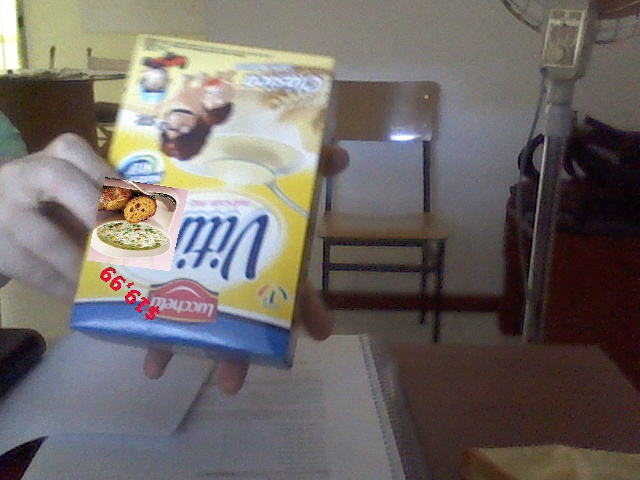
\includegraphics[width=0.33\textwidth]{../../imgvitina/captured87,000000}\label{fig:first_detect_protitpo}} \\
	\subfloat{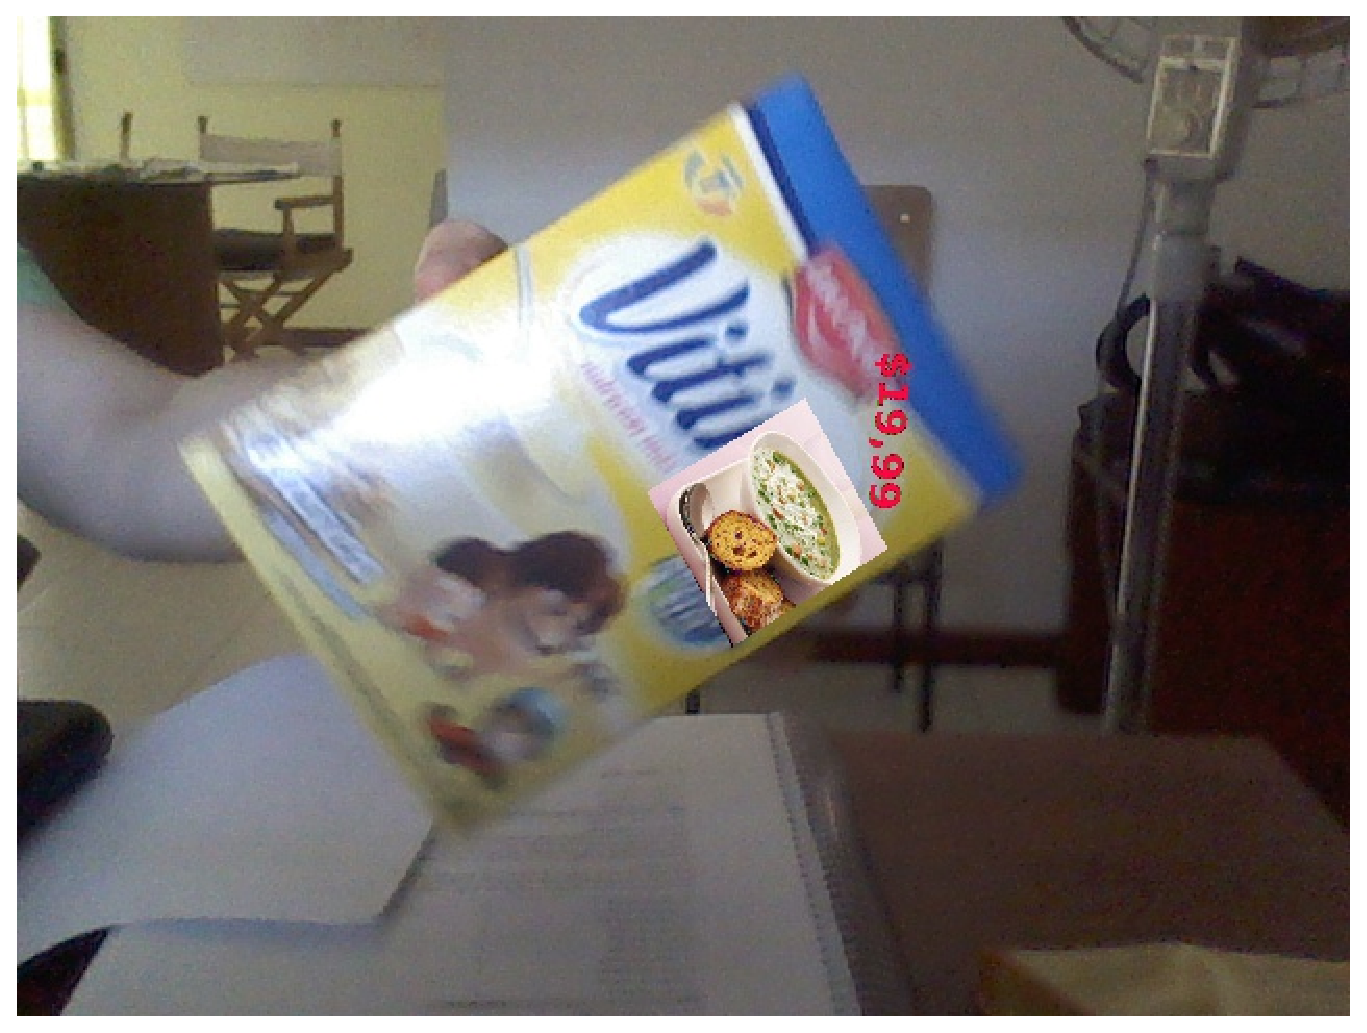
\includegraphics[width=0.33\textwidth]{../../imgvitina/captured94,000000}}
	% \subfloat[][]{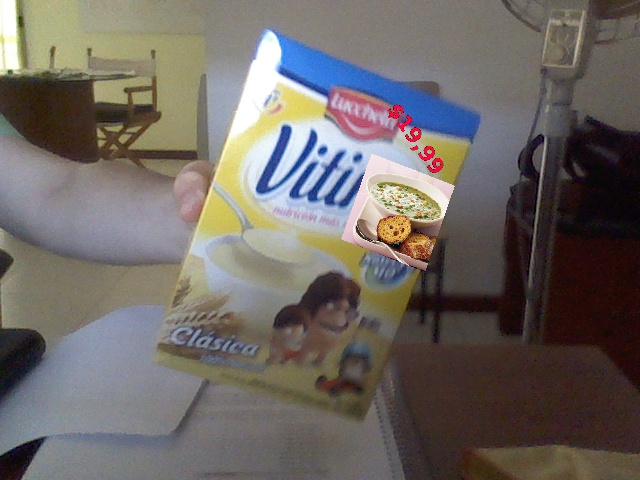
\includegraphics[width=2.5in]{../imgvitina/captured97,000000}}
	% \subfloat[][]{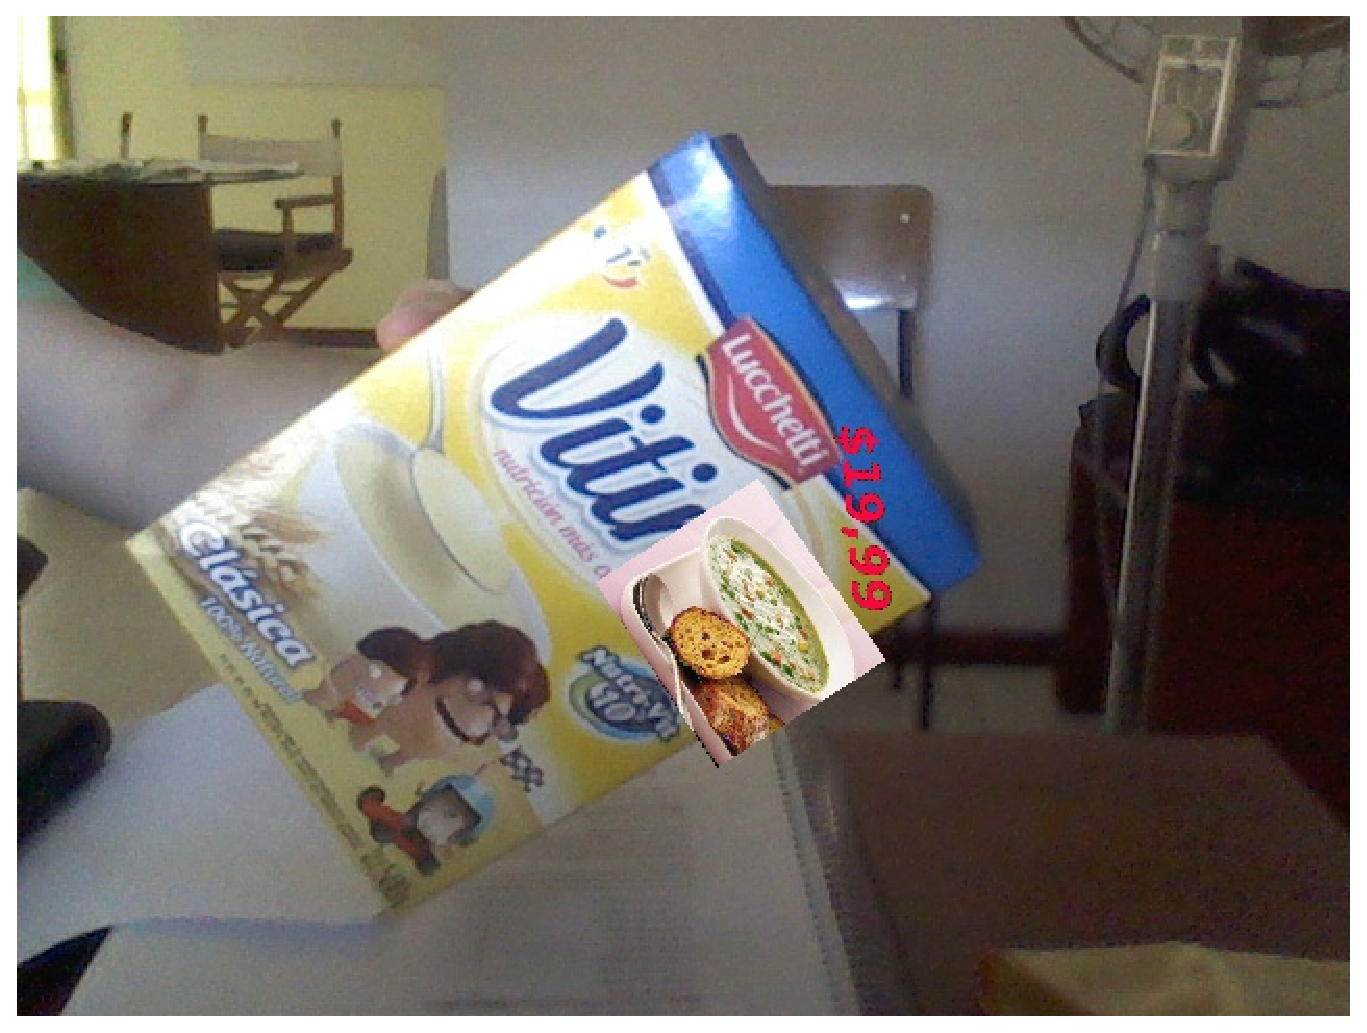
\includegraphics[width=2.5in]{../imgvitina/captured120,000000}}
	% \subfloat[][]{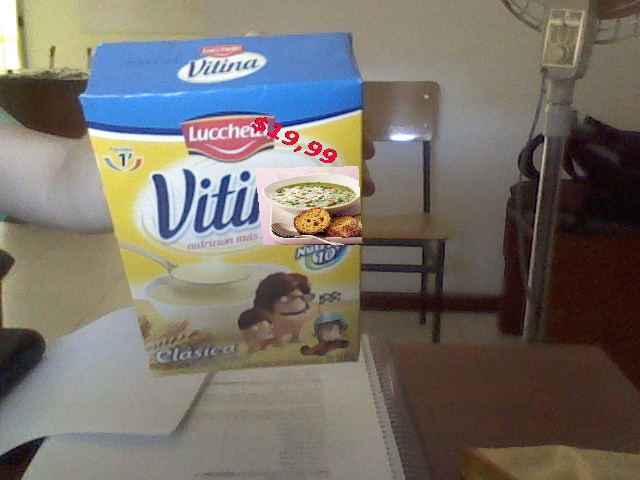
\includegraphics[width=2.5in]{../imgvitina/captured140,000000}}\\
	\subfloat{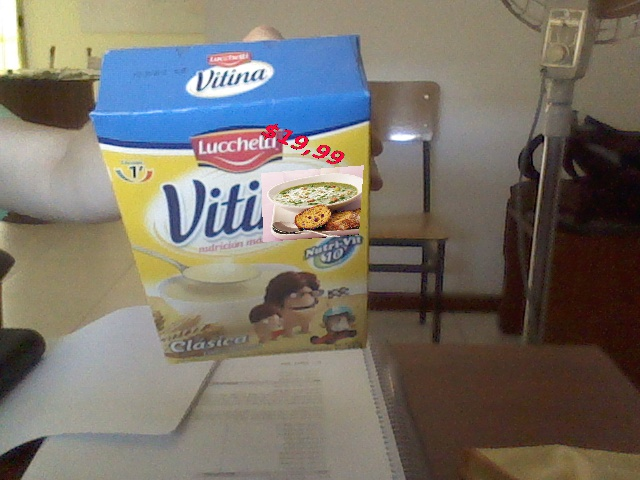
\includegraphics[width=0.33\textwidth]{../../imgvitina/captured146,000000}}
	% \subfloat[][]{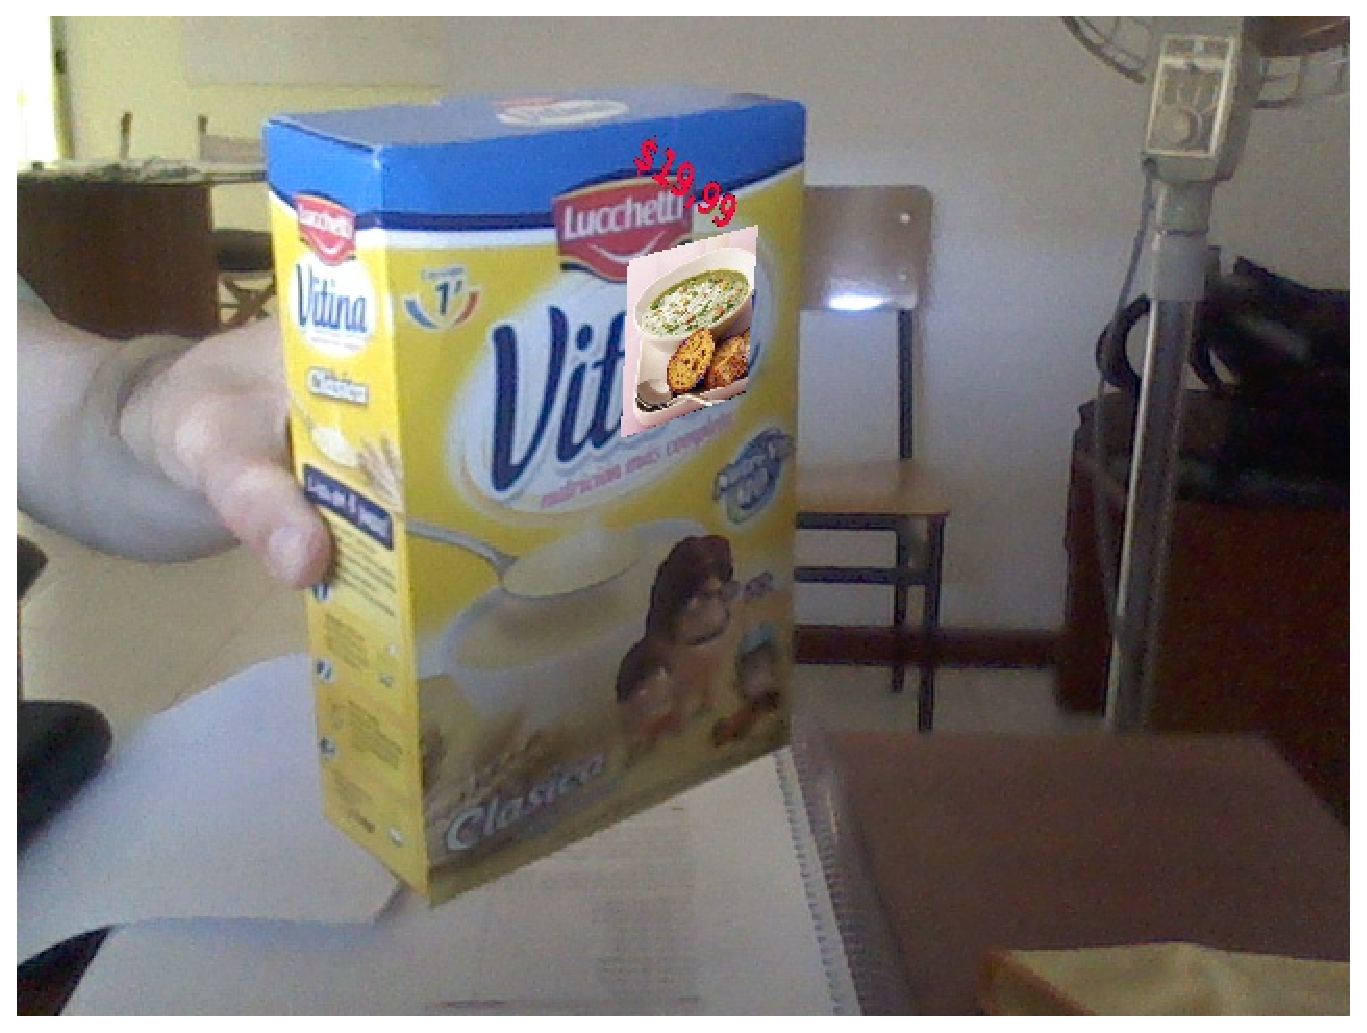
\includegraphics[width=2.5in]{../imgvitina/captured151,000000}}
	\subfloat{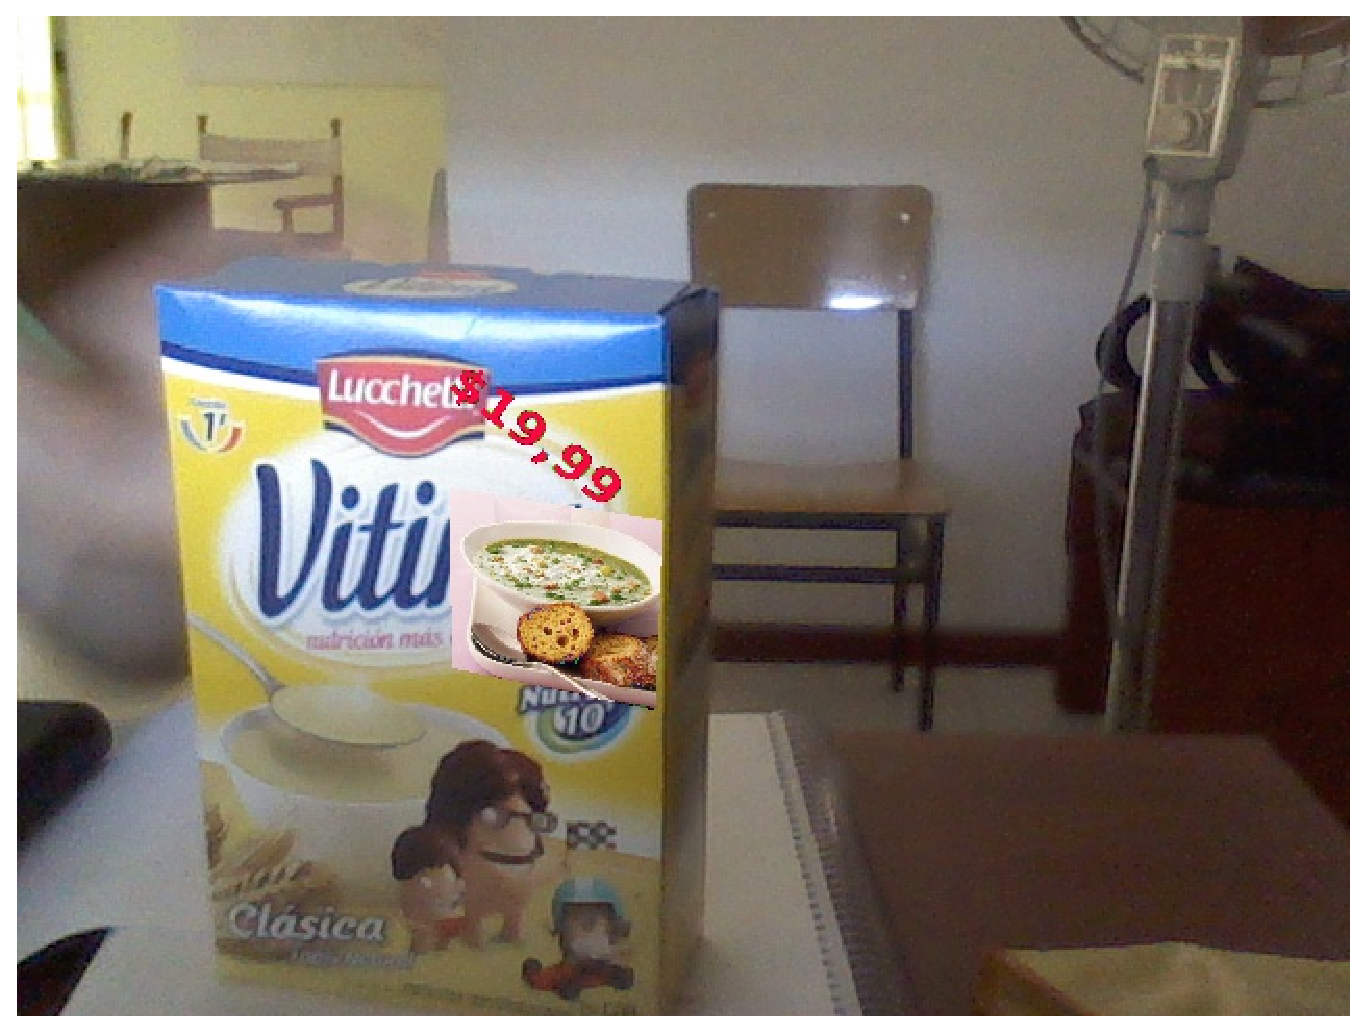
\includegraphics[width=0.33\textwidth]{../../imgvitina/captured176,000000}\label{fig:last_detect_prototipo}}
	\label{fig:ejemplos_protitipos}
    \end{figure}
    \note[item]{Marcelo: Imagen patrón, objeto de realidad aumentada a sobreimprimir en el flujo de video y diferentes capturas en la etapa de ejecución para el prototipo publicitario.}
    \note[item]{si bien se presentaron estos prototipos se pueden llevar a cabo otro tipo de acciones, reproducción de audio, denotar algo en el flujo de video, escribir instrucciones, etc. las posibilidades son infinitas.}
  \end{frame}
%   %mostrar videos:
%   \begin{frame}{Videos}
% %\movie[externalviewer]{placeholder box}{./img1/videos/preproc.mpeg}
% %\hyperlink{./img1/videos/preproc.mpeg}{\beamerbutton{Go somewhere}}
% \href{run:vlc /home/christian/Documentos/universidad/2011/codigo_e_informes/openCV/anteproyecto/tesis/pruebas_modif/3500_sinproc/out.ogv}{\beamerbutton{Prueba P1}}
% \href{run:vlc /home/christian/Documentos/universidad/2011/codigo_e_informes/openCV/anteproyecto/tesis/pruebas_modif/5000_sinproc/out.ogv}{\beamerbutton{Prueba P2}}
% \href{run:vlc /home/christian/Documentos/universidad/2011/codigo_e_informes/openCV/anteproyecto/tesis/pruebas_modif/vitina2-1.ogv}{\beamerbutton{Prototipo publicitario}}
% %\movie[width=3cm,height=2cm,poster]{}{./img1/videos/preproc.mpeg}
% \end{frame}